\section{Design and Implementation}
\subsection{Power Stage Calculation and Component Selection}
Design of a 500W Full-Bridge Converter Operating in Continuous Conduction Mode (CCM) with
the following specifications:
\begin{table}[h!]
    \centering
    \begin{tabular}{ll}
        \toprule
        \textbf{Parameter} & \textbf{Value} \\
        \midrule
        Input Voltage ($V_{\text{in}}$) & $\SI{310}{\volt}$ \\
        Duty Cycle ($D$) & $30\% $ \\
        Output Voltage ($V_{\text{out}}$) & $\SI{24}{\volt}$ \\
        Diode Voltage $(V_d)$ & $1V$\\
        Output Power ($P_{\text{out}}$) & $\SI{1000}{\watt}$ \\
        Switching Frequency ($f_{\text{sw}}$) & $\SI{100}{\kilo\hertz}$ \\
        Ripple Current Rated ($\Delta I_{\text{ripple}}$) & $30\%$ \\
        Ripple Voltage Rated ($\Delta V_{\text{ripple}}$) & $1\%$ \\
        Efficiency & $90\%$ \\
        \bottomrule
    \end{tabular}
    \caption{Input Parameters}
    \label{tab:system_parameters}
\end{table}
\subsection{Power Stage Calculation}

\subsubsection*{Transformer Turns Ratio (\(T\))}
\begin{equation}
T = \frac{2 \cdot V_{\text{in}} \cdot D}{V_{\text{out}} + 2 \cdot V_d} = \frac{2 \cdot 310 \cdot 0.3}{24 + 2 \cdot 1} = \frac{186}{26} \approx \boxed{7.15}
\end{equation}


\subsubsection*{Output Current (\(I_{\text{out}}\))}
\begin{equation}
I_{\text{out}} = \frac{P_{\text{out}}}{V_{\text{out}}} = \frac{1000}{24} \approx \boxed{41.67\;\text{A}}
\end{equation}

\subsubsection*{Load Resistance (\(R_L\))}
\begin{equation}
R_L = \frac{V_{\text{out}}^2}{P_{\text{out}}} = \frac{24^2}{1000} = \frac{576}{1000} = \boxed{0.576\;\Omega}
\end{equation}

\subsubsection*{Primary Voltage}
\begin{equation}
 V_p = \frac{V_{\text{in}}}{2} = \frac{310}{2} = \boxed{155\,\text{V}}
\end{equation}

\subsubsection*{Input Power (\(P_{\text{in}}\))}
\begin{equation}
P_{\text{in}} = \frac{P_{\text{out}}}{\eta} = \frac{1000}{0.9} \approx \boxed{1111.11\;\text{W}}
\end{equation}

\subsubsection*{Primary Average Current}
\begin{equation}
I_{p\_\text{avg}} = \frac{P_{\text{out}}}{\eta \cdot V_{\text{in}}} = \frac{1000}{0.9 \cdot 310} \approx \boxed{3.584\;\text{A}}
\end{equation}

\subsubsection*{Primary Ripple Current}
\begin{equation}
\Delta I_p = \text{Ripple\_I} \cdot I_{p\_\text{avg}} = 0.3 \cdot 3.584 \approx \boxed{1.075\;\text{A}}
\end{equation}

\subsubsection*{Primary Maximum Current}
\begin{equation}
I_{p\_\text{max}} = I_{p\_\text{avg}} + \frac{\Delta I_p}{2} = 3.584 + \frac{1.075}{2} \approx \boxed{4.122\;\text{A}}
\end{equation}

\subsubsection*{Primary Minimum Current}
\begin{equation}
I_{p\_\text{min}} = I_{p\_\text{max}} - \Delta I_p = 4.122 - 1.075 \approx \boxed{3.047\;\text{A}}
\end{equation}

\subsubsection*{Primary Inductance}
\begin{equation}
L_p = \frac{V_{\text{in}} \cdot D}{F_{\text{sw}} \cdot \Delta I_p} = \frac{310 \cdot 0.3}{100 \times 10^3 \cdot 1.075} \approx \boxed{865\;\mu\text{H}}
\end{equation}

\subsubsection*{Secondary Inductance}
\begin{equation}
L_s = \frac{L_p}{T^2} = \frac{865 \times 10^{-6}}{(7.15)^2} \approx \boxed{16.9\;\mu\text{H}}
\end{equation}

\subsubsection*{Output Ripple Current}
\begin{equation}
\Delta I_{\text{out}} = \text{Ripple\_I} \cdot I_{\text{out}} = 0.3 \cdot 41.67 \approx \boxed{12.5\;\text{A}}
\end{equation}

\subsubsection*{Output Maximum Current}
\begin{equation}
I_{\text{out\_max}} = I_{\text{out}} + \frac{\Delta I_{\text{out}}}{2} = 41.67 + \frac{12.5}{2} \approx \boxed{47.92\;\text{A}}
\end{equation}

\subsubsection*{Output Minimum Current}
\begin{equation}
I_{\text{out\_min}} = I_{\text{out}} - \frac{\Delta I_{\text{out}}}{2} = 41.67 - 6.25 \approx \boxed{35.42\;\text{A}}
\end{equation}

\subsubsection*{Output Inductor}
\begin{equation}
L_{\text{out}} = \frac{V_{\text{out}} \cdot D}{F_{\text{sw}} \cdot \Delta I_{\text{out}}} = \frac{24 \cdot 0.3}{100 \times 10^3 \cdot 12.5} \approx \boxed{5.76\;\mu\text{H}}
\end{equation}

\subsubsection*{Output Ripple Voltage (\(\Delta V_{\text{out}}\))}
\begin{equation}
\Delta V_{\text{out}} = \text{Ripple\_V} \cdot V_{\text{out}} = 0.01 \cdot 24 = \boxed{\SI{0.24}{\volt}}
\end{equation}

\subsubsection*{Output Capacitor}
\begin{equation}
C_{\text{out}} = \frac{I_{\text{out}} \cdot D}{F_{\text{sw}} \cdot \Delta V_{\text{out}}} = \frac{41.67 \cdot 0.3}{100 \times 10^3 \cdot 0.24} \approx \boxed{520.8\;\mu\text{F}}
\end{equation}

\subsubsection*{MOSFET Selection}
\begin{center}
    \begin{minipage}{0.4\textwidth}
        \centering
        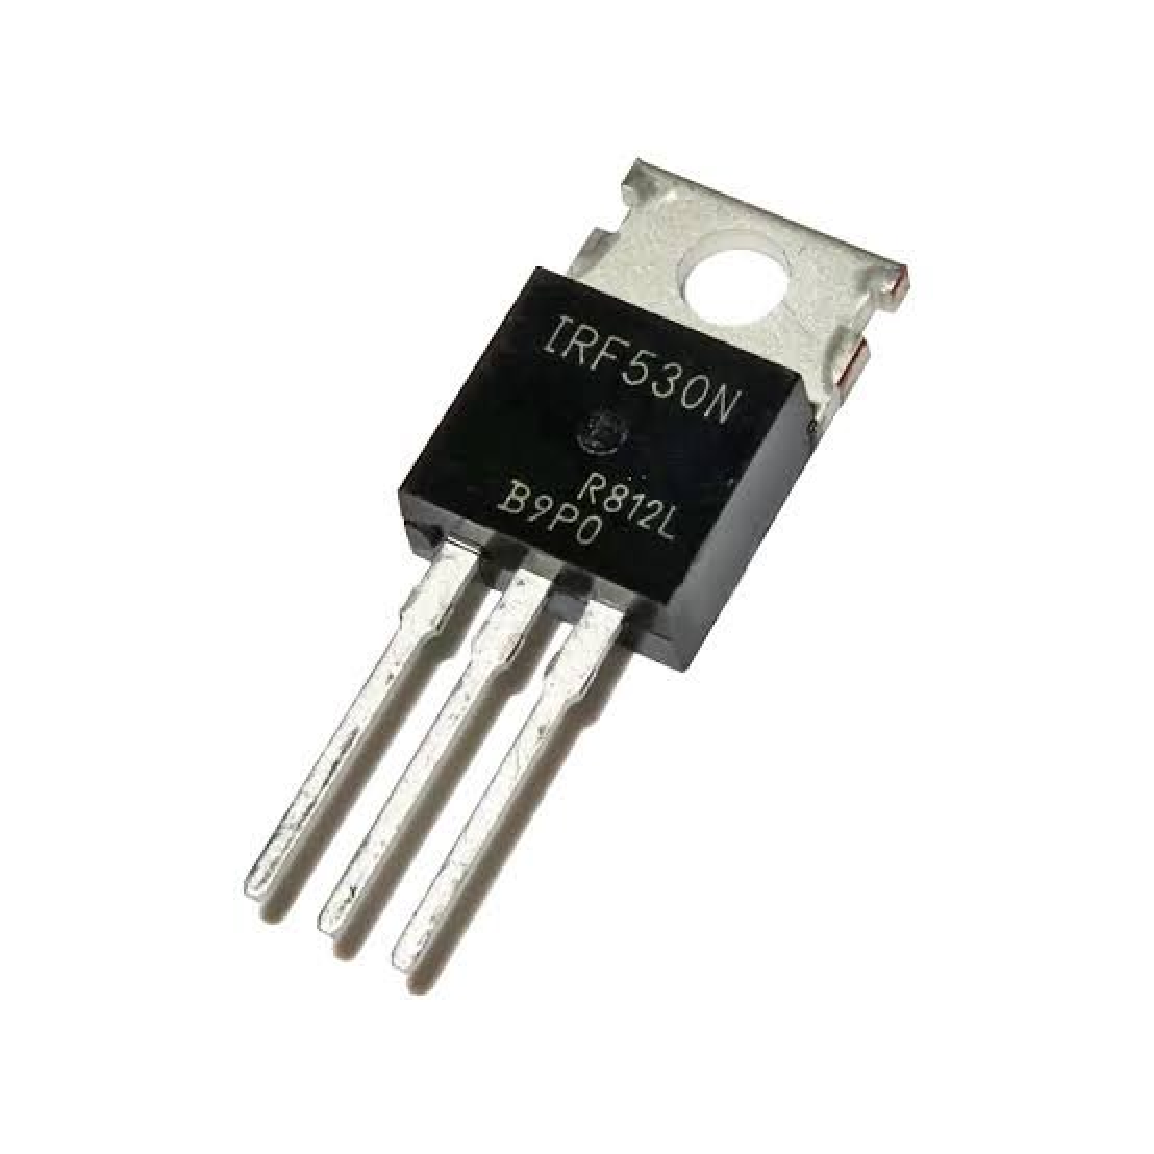
\includegraphics[width=0.8\linewidth]{Pictures/pics/mosfet.pdf} % Replace with your image file
        %\captionof{figure}{This is a figure.} % Add a caption
    \end{minipage}
    \hfill % Adds space between the minipages
    \begin{minipage}{0.55\textwidth}
    \centering
    \captionof{table}{STW11NM80 MOSFET}
    \label{tab:IRF530}
    \begin{tabular}{lcc}
    \toprule
    \footnotesize
    \textbf{Parameter} & \textbf{Value} & \textbf{Test Conditions} \\
    \midrule
     $V_{DS}$ & \SI{800}{\volt} & Absolute Maximum Rating \\
     $I_D$ & \SI{15}{\ampere} & $T_C = \SI{25}{\celsius}$ \\
     & \SI{10}{\ampere} & $T_C = \SI{100}{\celsius}$ \\
     $R_{DS(on)}$ & \SI{0.16}{\ohm} & $V_{GS} = \SI{10}{\volt}, I_D = \SI{8.4}{\ampere}$ \\
    \bottomrule
    \end{tabular}
    \end{minipage}
\end{center}
\subsubsection*{Diode Selection}
\begin{center}
    \begin{minipage}{0.4\textwidth}
        \centering
        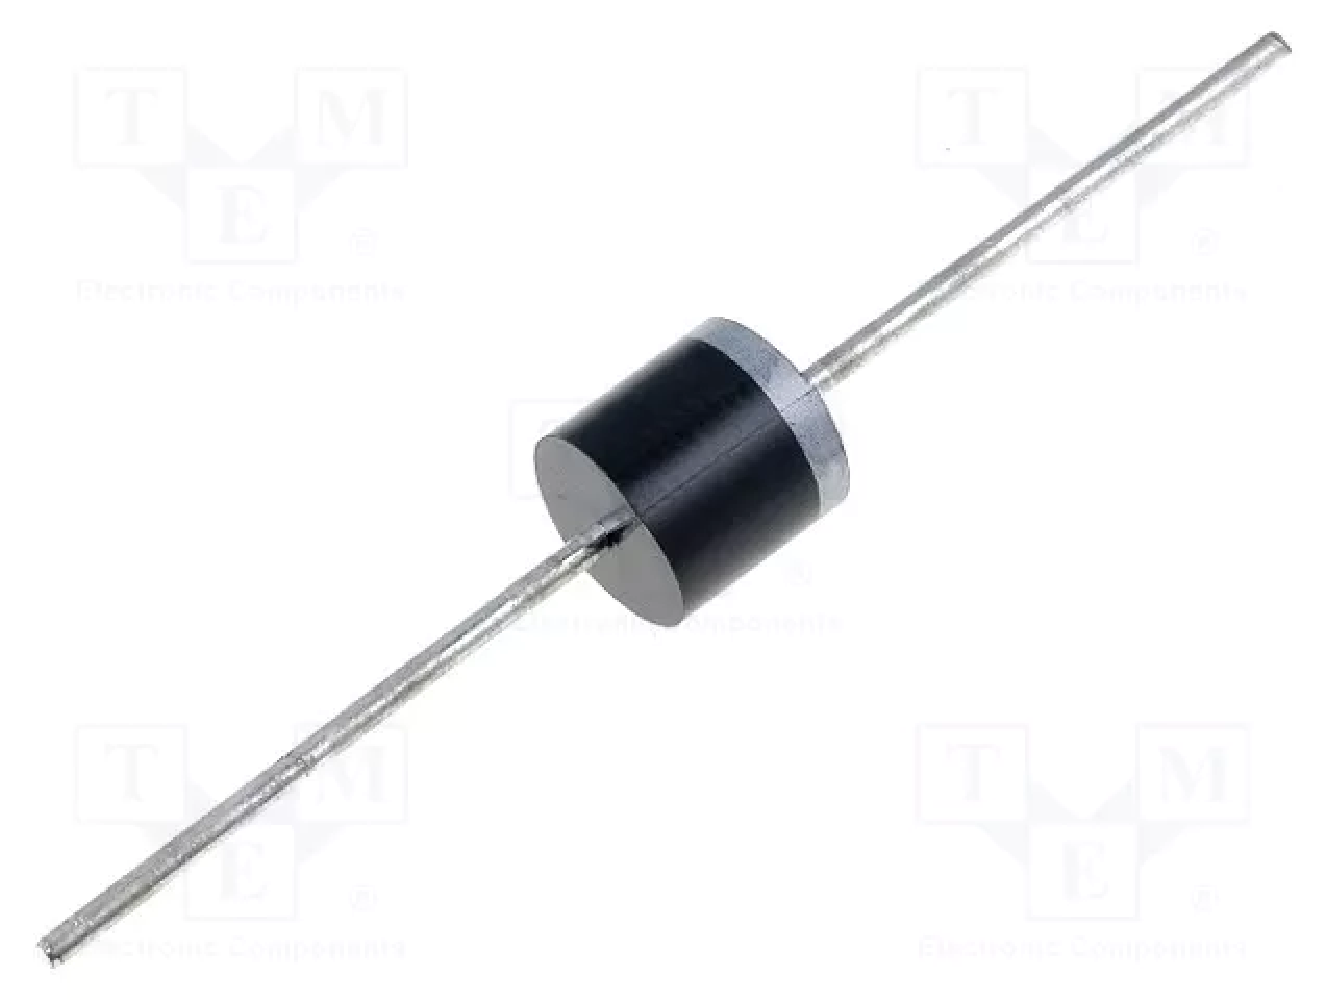
\includegraphics[width=0.7\linewidth]{Pictures/pics/diode.pdf} % Replace with your image file
        %\captionof{figure}{This is a figure.} % Add a caption
    \end{minipage}
    \hfill % Adds space between the minipages
    \begin{minipage}{0.55\textwidth}
    \centering
    \captionof{table}{VS-E5PX6012 Diode}
        \label{tab:SR510}
        \begin{tabular}{lcc}
        \toprule
        \textbf{Parameter} & \textbf{Value} & \textbf{Test Conditions} \\
        \midrule
        $V_{RRM}$ & \SI{1000}{\volt} & Maximum repetitive rating \\
        $I_F$ & \SI{60}{\ampere} & Continuous, $T_A = \SI{25}{\celsius}$ \\
        \bottomrule
        \end{tabular}
    \end{minipage}
\end{center}
\subsection{Transformer Design}
\begin{table}[h]
\centering
\caption{Design Parameters for Transformer Core Calculation}
\label{tab:parameters}
\begin{tabular}{lll}
\toprule
\textbf{Parameter} & \textbf{Value} & \textbf{Description} \\
\midrule
\texttt{Pout} & \SI{1000}{\watt} & Output Power \\
\texttt{Vin} & \SI{310}{\volt} & Input Voltage \\
\texttt{U} & 1.41 & Center-tap winding factor \\
\texttt{n} & 0.9 & Efficiency (90\%) \\
\texttt{Kf} & 4 & Square wave form factor \\
\texttt{Bm} & \SI{0.05}{\tesla} & Flux density \\
\texttt{Fsw} & \SI{100}{\kilo\hertz} & Switching frequency \\
\texttt{alpha} & 0.5 & Regulation factor \\
\texttt{Ku} & 0.4 & Window utilization \\
\texttt{D} & 0.3 & Duty cycle \\
\texttt{Iout} & \SI{41.67}{\ampere} & Output current \\
\bottomrule
\end{tabular}
\end{table}

\subsubsection*{Secondary Apparent Power (\(P_t\))}
\begin{equation}
P_t = \left(\frac{P_{out}}{\eta}\right) \cdot U + P_{out} \cdot U 
    = \left(\frac{1000}{0.9}\right) \cdot 1.41 + 1000 \cdot 1.41 
    = \boxed{2976.67\;\text{VA}}
\end{equation}


\subsubsection*{Electrical Condition (\(K_e\))}
\begin{equation}
K_e = 0.145 \cdot K_f^2 \cdot F_{sw}^2 \cdot B_m^2 \cdot 10^{-4} 
    = 0.145 \cdot (4)^2 \cdot (100 \times 10^3)^2 \cdot (0.05)^2 \cdot 10^{-4} 
    = \boxed{5800}
\end{equation}

\subsubsection*{Core Geometry (\(K_g\))}
\begin{equation}
K_g = \left(\frac{P_t}{2 \cdot K_e \cdot \alpha}\right) \cdot 1.35 
    = \left(\frac{2976.67}{2 \cdot 5800 \cdot 0.5}\right) \cdot 1.35 
    = \boxed{0.6928\;\text{cm}^5}
\end{equation}


\begin{figure}[h!]
    \centering
    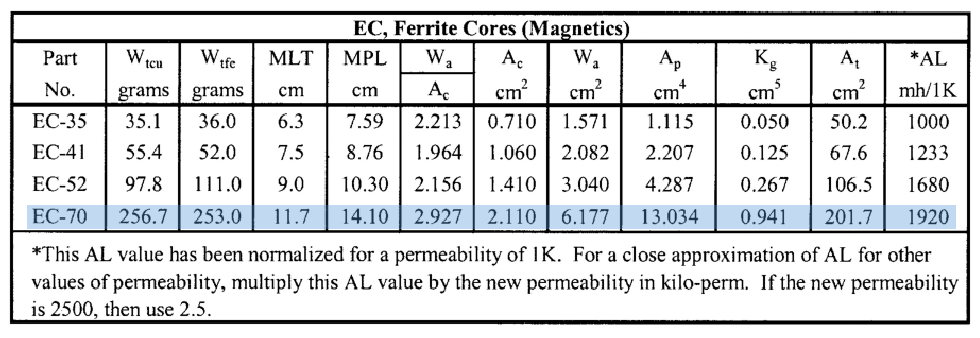
\includegraphics[width=1\linewidth]{Pictures/image/EC-70_table.pdf}
    \caption{\textcolor{blue}{\textit{\footnotesize EC Core Parameter Table List}}}
\end{figure} 
\begin{figure}[h!]
    \centering
    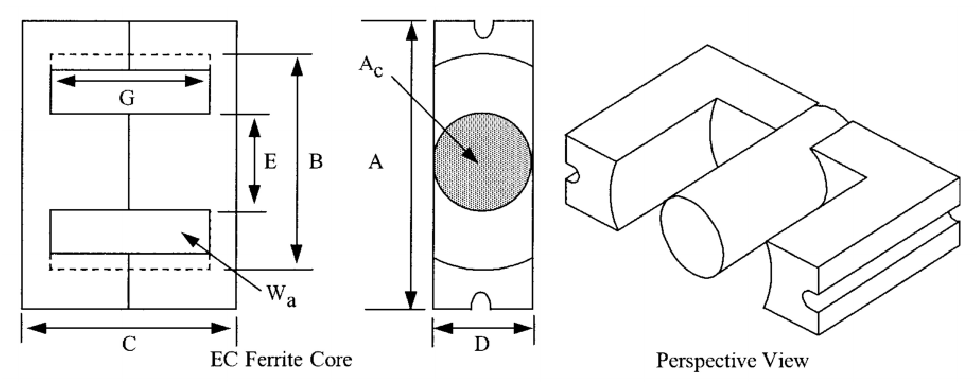
\includegraphics[width=1\linewidth]{Pictures/image/EC-70_structure.pdf}
    \caption{\textcolor{blue}{\textit{\footnotesize EC-70 Core}}}
\end{figure} 

\begin{table}[h!]
\centering
\begin{tabular}{l l l}
\toprule
\textbf{Parameter} & \textbf{Value} & \textbf{Unit} \\
\midrule
Magnetic Path Length ($MPL$) & $\SI{14.10}{}$ & \si{\centi\meter} \\
Core Weight ($W_{\text{core}}$) & $\SI{253}{}$ & \si{\gram} \\
Copper Weight ($W_{\text{copper}}$) & $\SI{256.7}{}$ & \si{\gram} \\
Mean Length Turn ($MLT$) & $\SI{11.7}{}$ & \si{\centi\meter} \\
Cross-Sectional Area ($A_c$) & $\SI{2.11}{}$ & \si{\centi\meter\squared} \\
Window Area ($W_a$) & $\SI{6.177}{}$ & \si{\centi\meter\squared} \\
Core Product ($A_p$) & $\SI{13.034}{}$ & \si{\centi\meter\tothe{4}} \\
Core Geometry ($K_{gs}$) & $\SI{0.941}{}$ & \si{\centi\meter\tothe{5}} \\
\bottomrule
\end{tabular}
\caption{Selected Core Parameters for Transformer Design}
\label{tab:core_parameters}
\end{table}

\subsubsection*{Current Density (\(J\))}
\begin{equation}
J = \frac{P_t \cdot 10^4}{K_f \cdot K_u \cdot B_m \cdot F_{sw} \cdot A_p} 
  = \frac{2976.67 \cdot 10^4}{4 \cdot 0.4 \cdot 0.05 \cdot 100 \times 10^3 \cdot 13.034} 
  = \boxed{285.5\;\frac{\text{A}}{\text{cm}^2}}
\end{equation}

\subsubsection*{Primary Turns (\(N_p\))}
\begin{equation}
N_p = \frac{V_{in} \cdot 10^4}{K_f \cdot B_m \cdot F_{sw} \cdot A_c} 
    = \frac{310 \cdot 10^4}{4 \cdot 0.05 \cdot 100 \times 10^3 \cdot 2.11} 
    = \boxed{73.5\;\text{turns}}
\end{equation}

\subsubsection*{Input Current (\(I_{in}\))}
\begin{equation}
I_{in} = \frac{P_{out}}{\eta \cdot V_{in}} 
       = \frac{1000}{0.9 \cdot 310} 
       = \boxed{3.584\;\text{A}}
\end{equation}

\subsubsection*{Primary Bare Wire Area (\(A_{pw}\))}
\begin{equation}
A_{pw} = \frac{I_{in} \cdot \sqrt{D}}{J} 
       = \frac{3.584 \cdot \sqrt{0.3}}{285.5} 
       = \boxed{6.88\;\text{mm}^2}
\end{equation}

\subsubsection*{Secondary Voltage}
\begin{equation}
    V_s = \frac{V_{\text{in}}}{7.15} = \frac{310}{7.15} \approx \boxed{43.36\,\text{V}}
\end{equation}

\subsubsection*{Secondary  Turn \( N_s\)}
\begin{equation}
    N_s = \left( \frac{N_p \cdot V_s}{V_{\text{in}}} \right) \cdot \left( 1 + \frac{\alpha}{100} \right) = \left( \frac{89 \cdot 43.36}{310} \right) \cdot 1.005 = \approx \boxed{10.32\,\text{turns}}
\end{equation}

\subsubsection*{Secondary Wire Area}
\begin{equation}
A_{\text{sw}} = \frac{I_{\text{out}} \cdot \sqrt{D}}{J} 
= \frac{41.67 \cdot \sqrt{0.3}}{383.4}
\approx \boxed{0.08\,\text{cm}^2}
\end{equation}
\subsection{Inductor Design}
\begin{table}[h]
\centering
\caption{Design Parameters for Ferrite Core Selection Using \( K_g \) Method}
\label{tab:core_parameters}
\begin{tabular}{llSS}
\toprule
\textbf{Parameter} & \textbf{Symbol} & \textbf{Value} & \textbf{Unit} \\
\midrule
Inductance & \( L \) & 5.76 & \si{\micro\henry} \\
DC Current & \( I_o \) & 41.6667 & \si{\ampere} \\
AC Current & \( \Delta I \) & 12.5 & \si{\ampere} \\
Output Power & \( P_o \) & 1000 & \si{\watt} \\
Regulation & \( \alpha \) & 1 & \% \\
Ripple Frequency & \( F_s \) & 100 & \si{\kilo\hertz} \\
Flux Density & \( B_m \) & 0.25 & \si{\tesla} \\
Window Utilization & \( K_u \) & 0.4 & \text{Dimensionless} \\
Temperature Rise & \( T_r \) & 25 & \si{\degreeCelsius} \\
\bottomrule
\end{tabular}
\end{table}
\subsubsection*{Peak Current}
\begin{equation}
I_{\text{pk}} = I_o + \frac{\Delta I}{2} 
= 41.6667 + \frac{12.5}{2}
= \boxed{47.92\,\text{A}}
\end{equation}

\subsubsection*{Energy-Handling}
\begin{equation}
E = \frac{L \cdot I_{\text{pk}}^2}{2} 
= \frac{1}{2} \cdot 5.76 \times 10^{-6}\ \text{H} \cdot (47.92\ \text{A})^2 
\boxed{0.0066\;\text{J}}
\end{equation}

\subsubsection*{Electrical Coefficient}
\begin{equation}
 K_e = 0.145 \cdot P_o \cdot B_m^2 \cdot 10^{-4} 
=  0.145 \cdot 1000\;\text{W} \cdot (0.25\;\text{T})^2 \cdot 10^{-4}
=  \boxed{0.000906}
\end{equation}

\subsubsection*{Core Geometry}
\begin{equation}
K_g = \frac{E^2}{K_e \cdot \alpha} 
= \frac{(0.0066\;\text{J})^2}{0.000906 \cdot 1} 
= \boxed{0.0483\;\text{cm}^5}   
\end{equation}

\begin{figure}[h!]
    \centering
    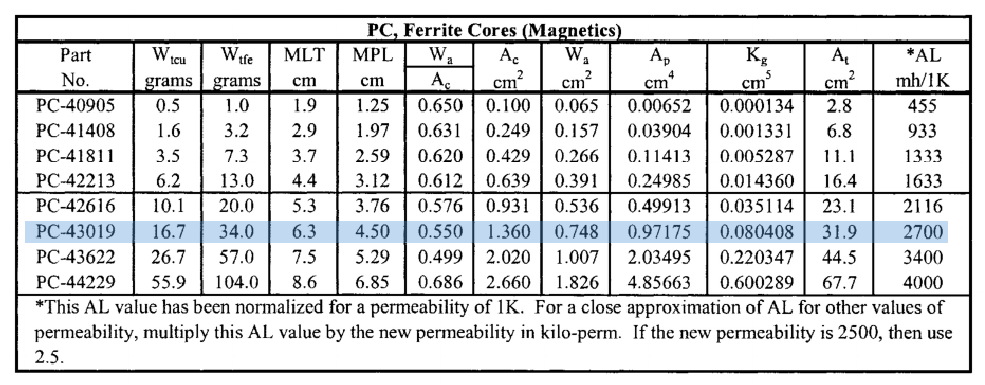
\includegraphics[width=1\linewidth]{Pictures/image/PC-43622_table.pdf}
    \caption{\textcolor{blue}{\textit{\footnotesize PC Core Parameter Table List}}}
\end{figure} 

\begin{figure}[h!]
    \centering
    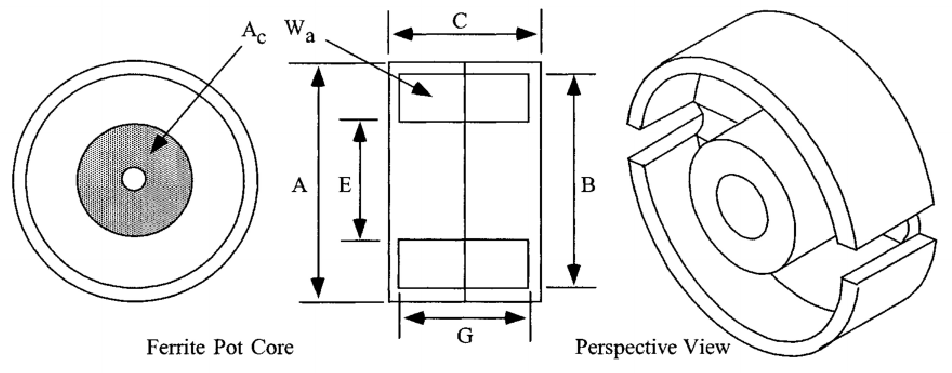
\includegraphics[width=1\linewidth]{Pictures/image/PC-43622_structure.pdf}
    \caption{\textcolor{blue}{\textit{\footnotesize PC-43019 Core}}}
\end{figure} 
\begin{table}[h]
\centering
\caption{EE-375 Ferrite Core Parameters}
\label{tab:EE16_parameters}
\begin{tabular}{llSS}
\toprule
\textbf{Parameter} & \textbf{Symbol} & \textbf{Value} & \textbf{Unit} \\
\midrule
Magnetic Path Length & \( \text{MPL} \) & 4.50 & \si{\centi\meter} \\
Core Weight & \( \text{We} \) & 34 & \si{\gram} \\
Mean Length Turn & \( \text{MLT} \) & 6.3 & \si{\centi\meter} \\
Cross-Sectional Area & \( A_c \) & 1.36 & \si{\centi\meter\squared} \\
Window Area & \( W_a \) & 0.748 & \si{\centi\meter\squared} \\
Core Product & \( A_p \) & 0.9717 & \si{\centi\meter\tothe{4}} \\
Core Geometry & \( K_g \) & 0.0804 & \si{\centi\meter\tothe{5}} \\
\bottomrule
\end{tabular}
\end{table}
\subsubsection*{Current Density}
\begin{equation}
J = \frac{2 \cdot E \cdot 10^4}{B_m \cdot A_p \cdot K_u} 
  = \frac{2 \cdot 0.0066 \cdot 10^4}{0.25 \cdot 0.9717 \cdot 0.4} 
  = \boxed{1361\;\frac{\text{A}}{\text{cm}^2}}
\end{equation}

\subsubsection*{RMS Current}
\begin{equation}
I_{rms} = \sqrt{I_o^2 + \Delta I^2} 
        = \sqrt{(41.67)^2 + (12.5)^2} 
        = \boxed{43.5\;\text{A}}
\end{equation}

\subsubsection*{Bare Wire Area}
\begin{equation}
A_w = \frac{I_{rms}}{J} 
    = \frac{43.5\;\text{A}}{1361\;\frac{\text{A}}{\text{cm}^2}} 
    = \boxed{0.032\;\text{cm}^2}
\end{equation}
\subsubsection*{Selected Wire Area}
\[
A_{ws} = 0.04\ \text{cm}^2
\]
\subsubsection*{Effective Window Area}
\begin{itemize}
    \item $S_3 = 0.75$ Window Effective factor for Ferrite core
\end{itemize}
\begin{equation}
W_{aeff} = W_a \cdot S_3 
         = 0.748\;\text{cm}^2 \cdot 0.75 
         = \boxed{0.561\;\text{cm}^2}
\end{equation}
\subsubsection*{Number of Turn}
\begin{itemize}
    \item $S_2 = 0.6$ Fill Factor 
\end{itemize}
\begin{equation}
N = \frac{W_{aeff} \cdot S_2}{A_{ws}} 
  = \frac{0.561\;\text{cm}^2 \cdot 0.6}{0.04\;\text{cm}^2}
  = \boxed{8.4\;\text{turns}} \quad (\text{Round to } 8\;\text{turns})
\end{equation}

\subsubsection*{Required Air Gap}
\begin{equation}
L_g = \frac{0.4 \pi N^2 A_c \cdot 10^{-8}}{L} - \frac{MPL}{\mu_0} 
    = \frac{0.4 \pi \cdot 8^2 \cdot 1.36 \cdot 10^{-8}}{5.76 \times 10^{-6}} - \frac{4.5}{2500}
    = \boxed{0.12\;\text{mm}}
\end{equation}


\newpage
\subsection{Simulation On LTspice}
\begin{figure}[h!]
    \centering
    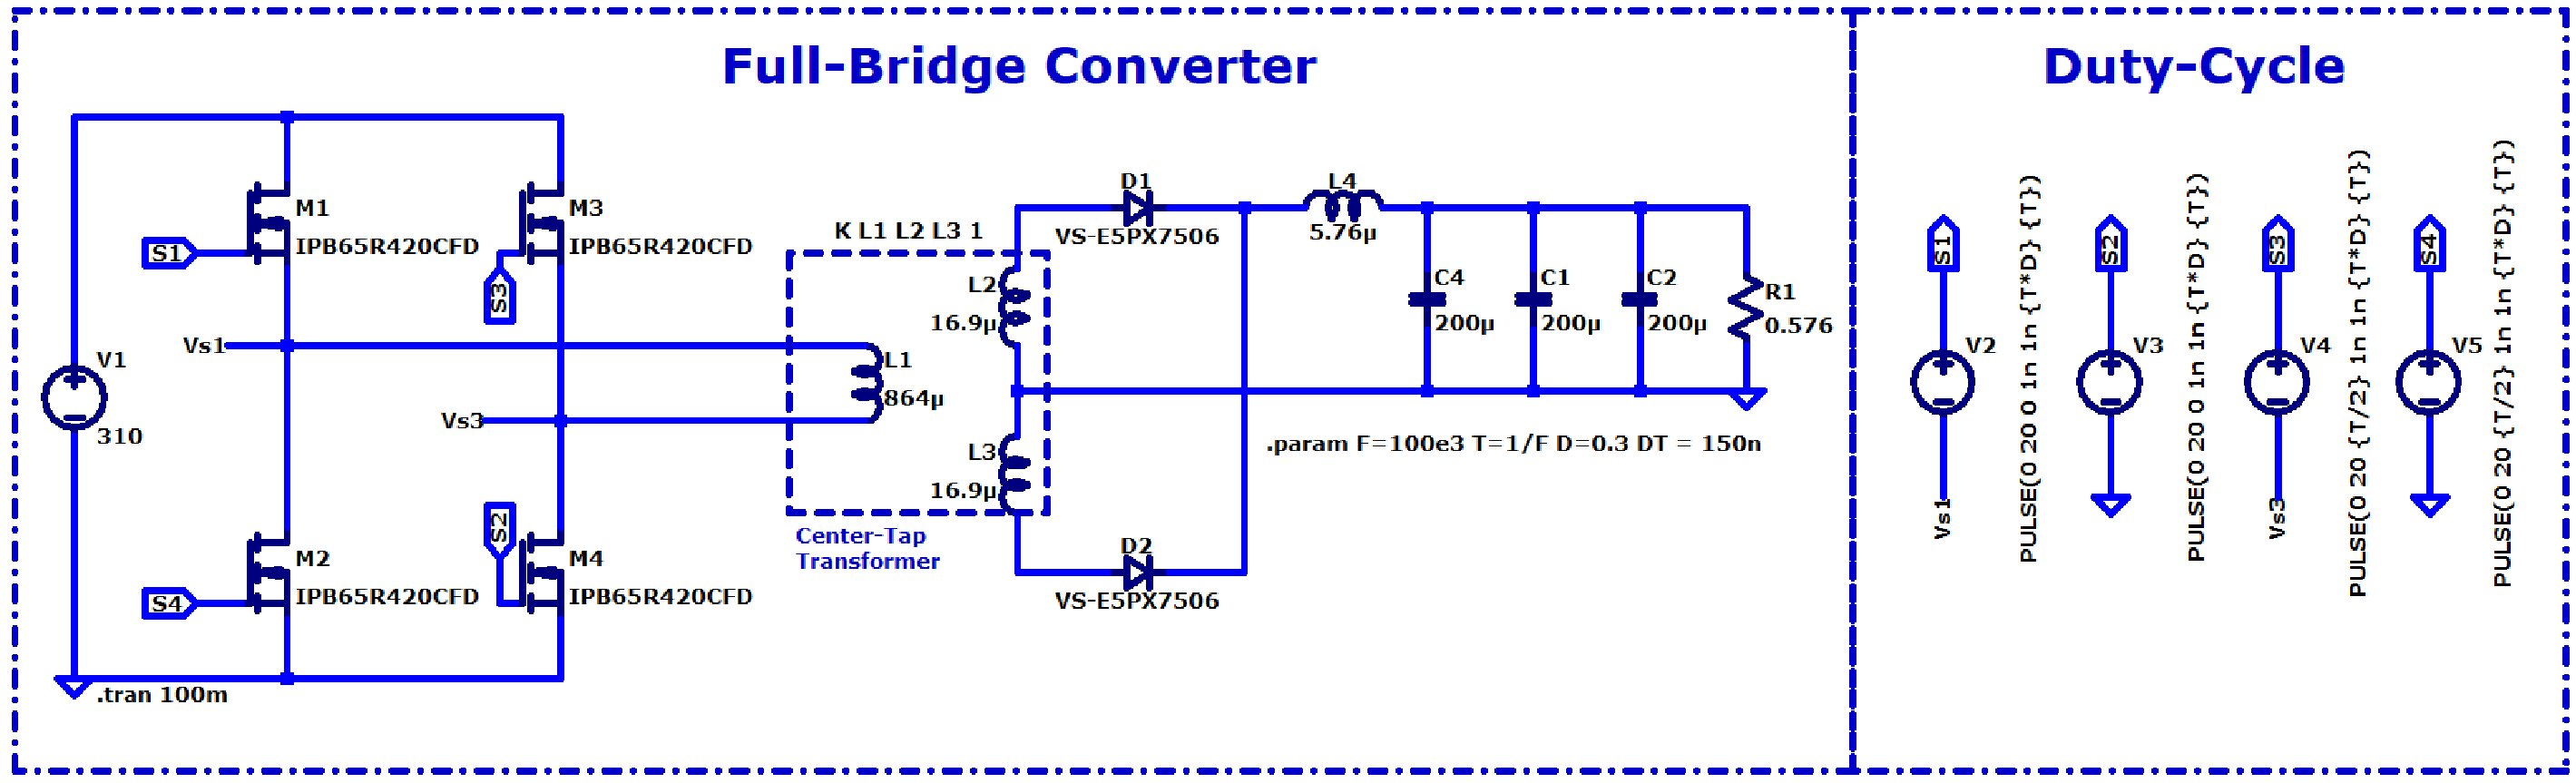
\includegraphics[width=1\linewidth]{Pictures/image/schem.pdf}
    \caption{\textcolor{blue}{\textit{\footnotesize Full-Bridge Converter Schematic on LTspice}}}
\end{figure}
\begin{figure}[h!]
    \centering
    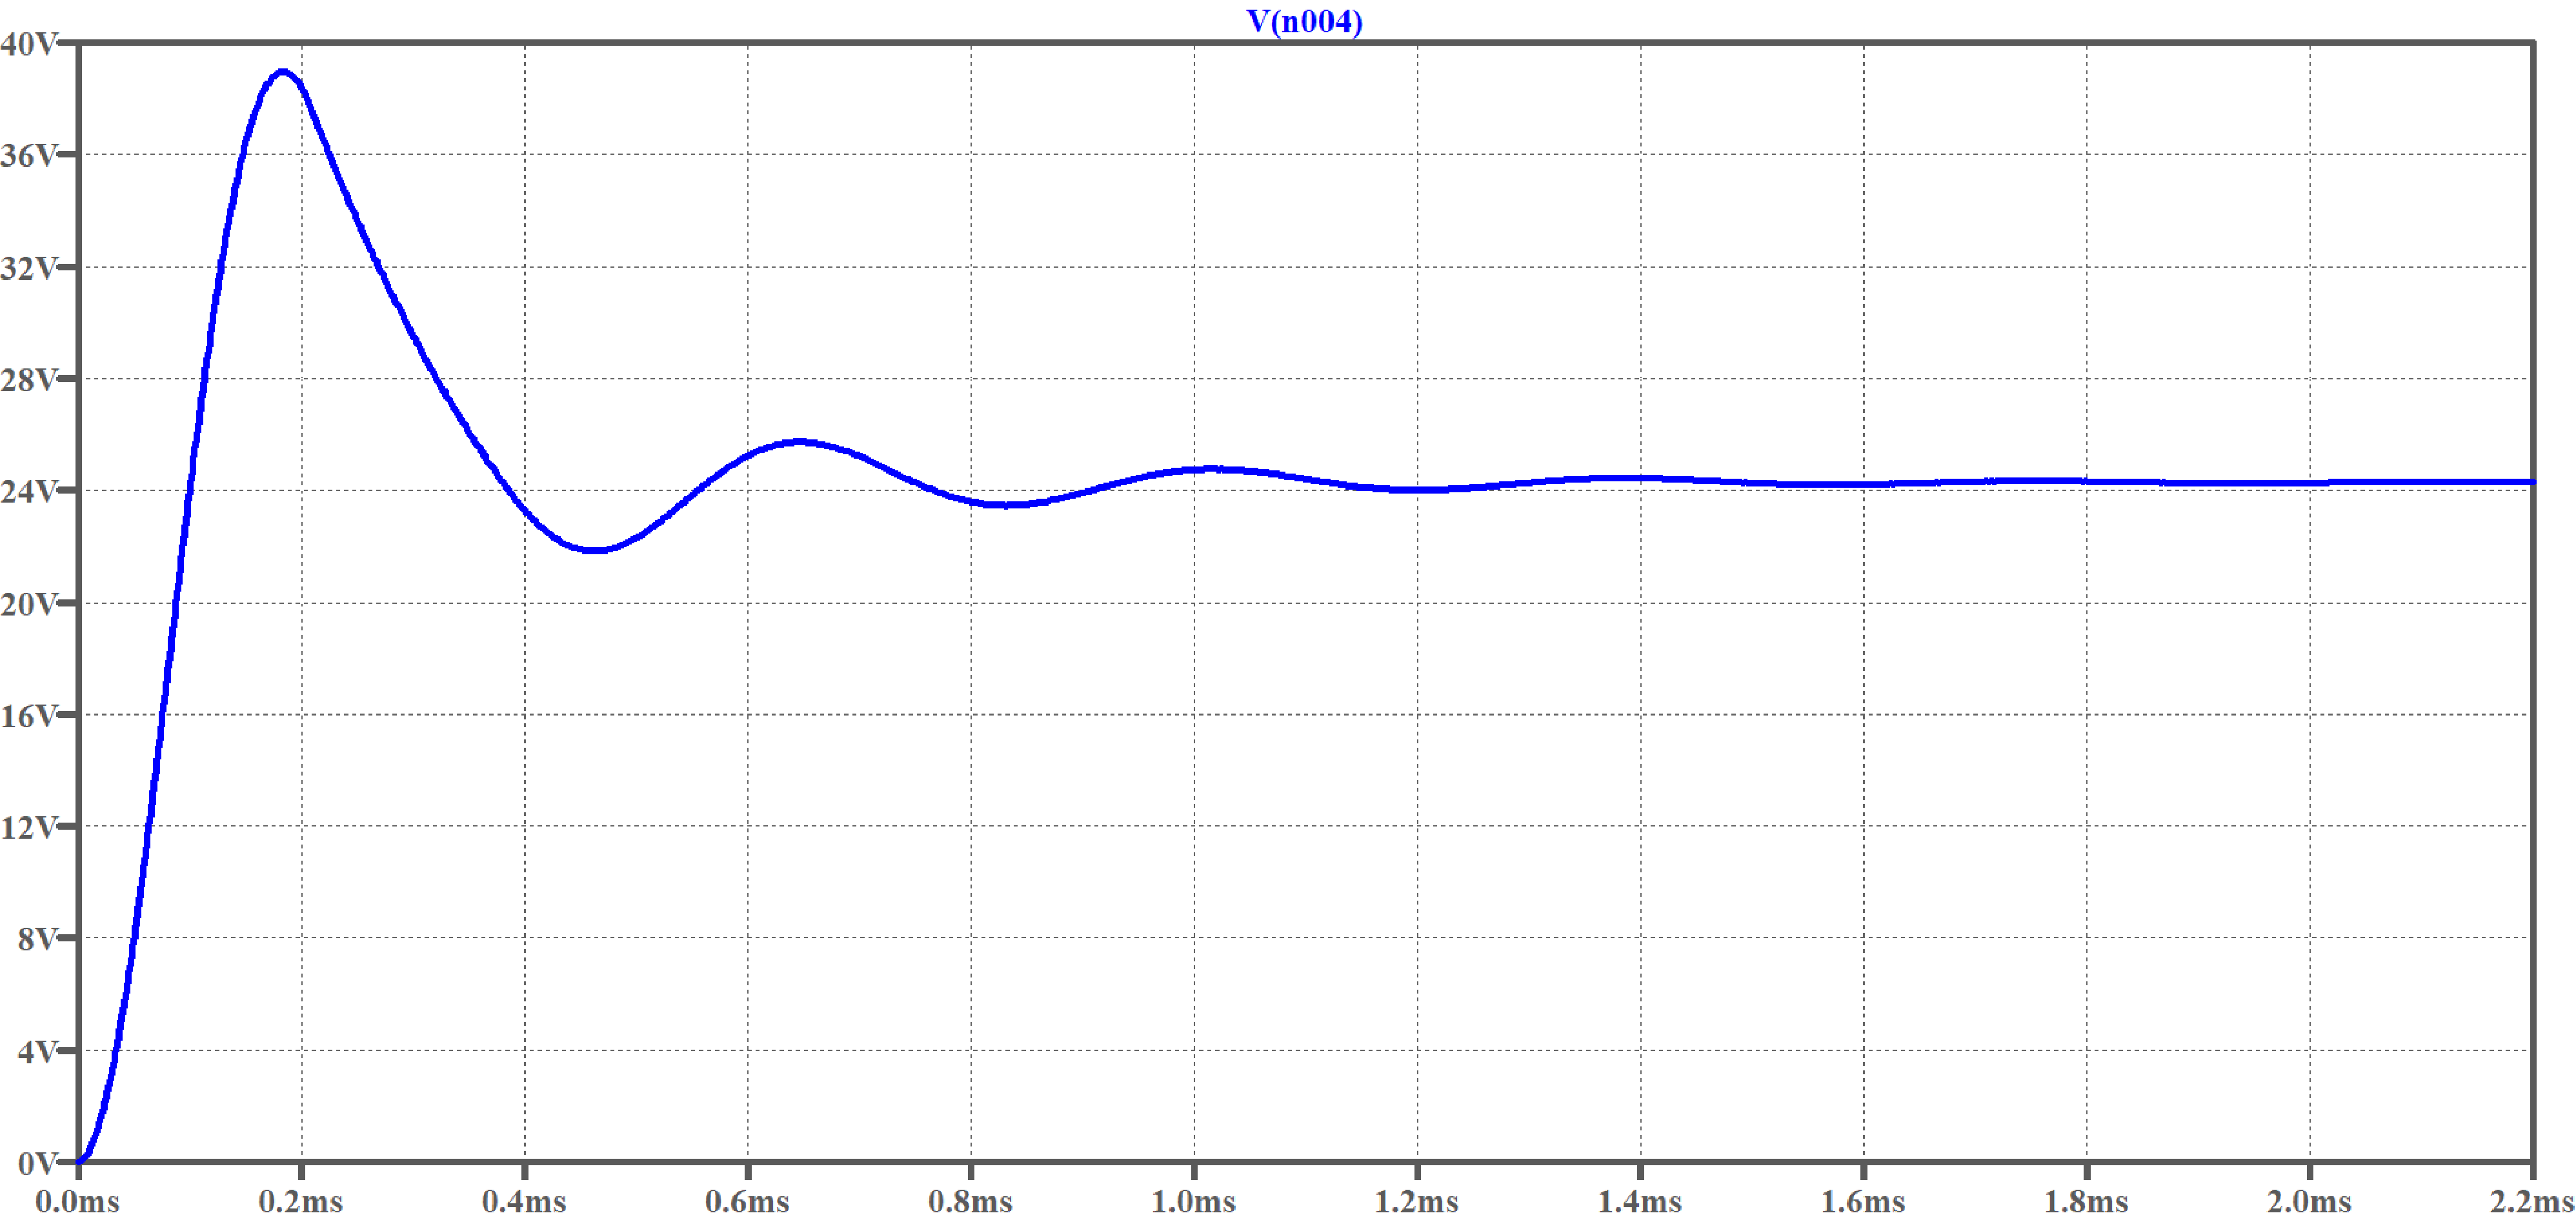
\includegraphics[width=0.8\linewidth]{Pictures/image/output_voltage.pdf}
    \caption{\textcolor{blue}{\textit{\footnotesize Output Voltage Waveform}}}
\end{figure}
\begin{figure}[h!]
    \centering
    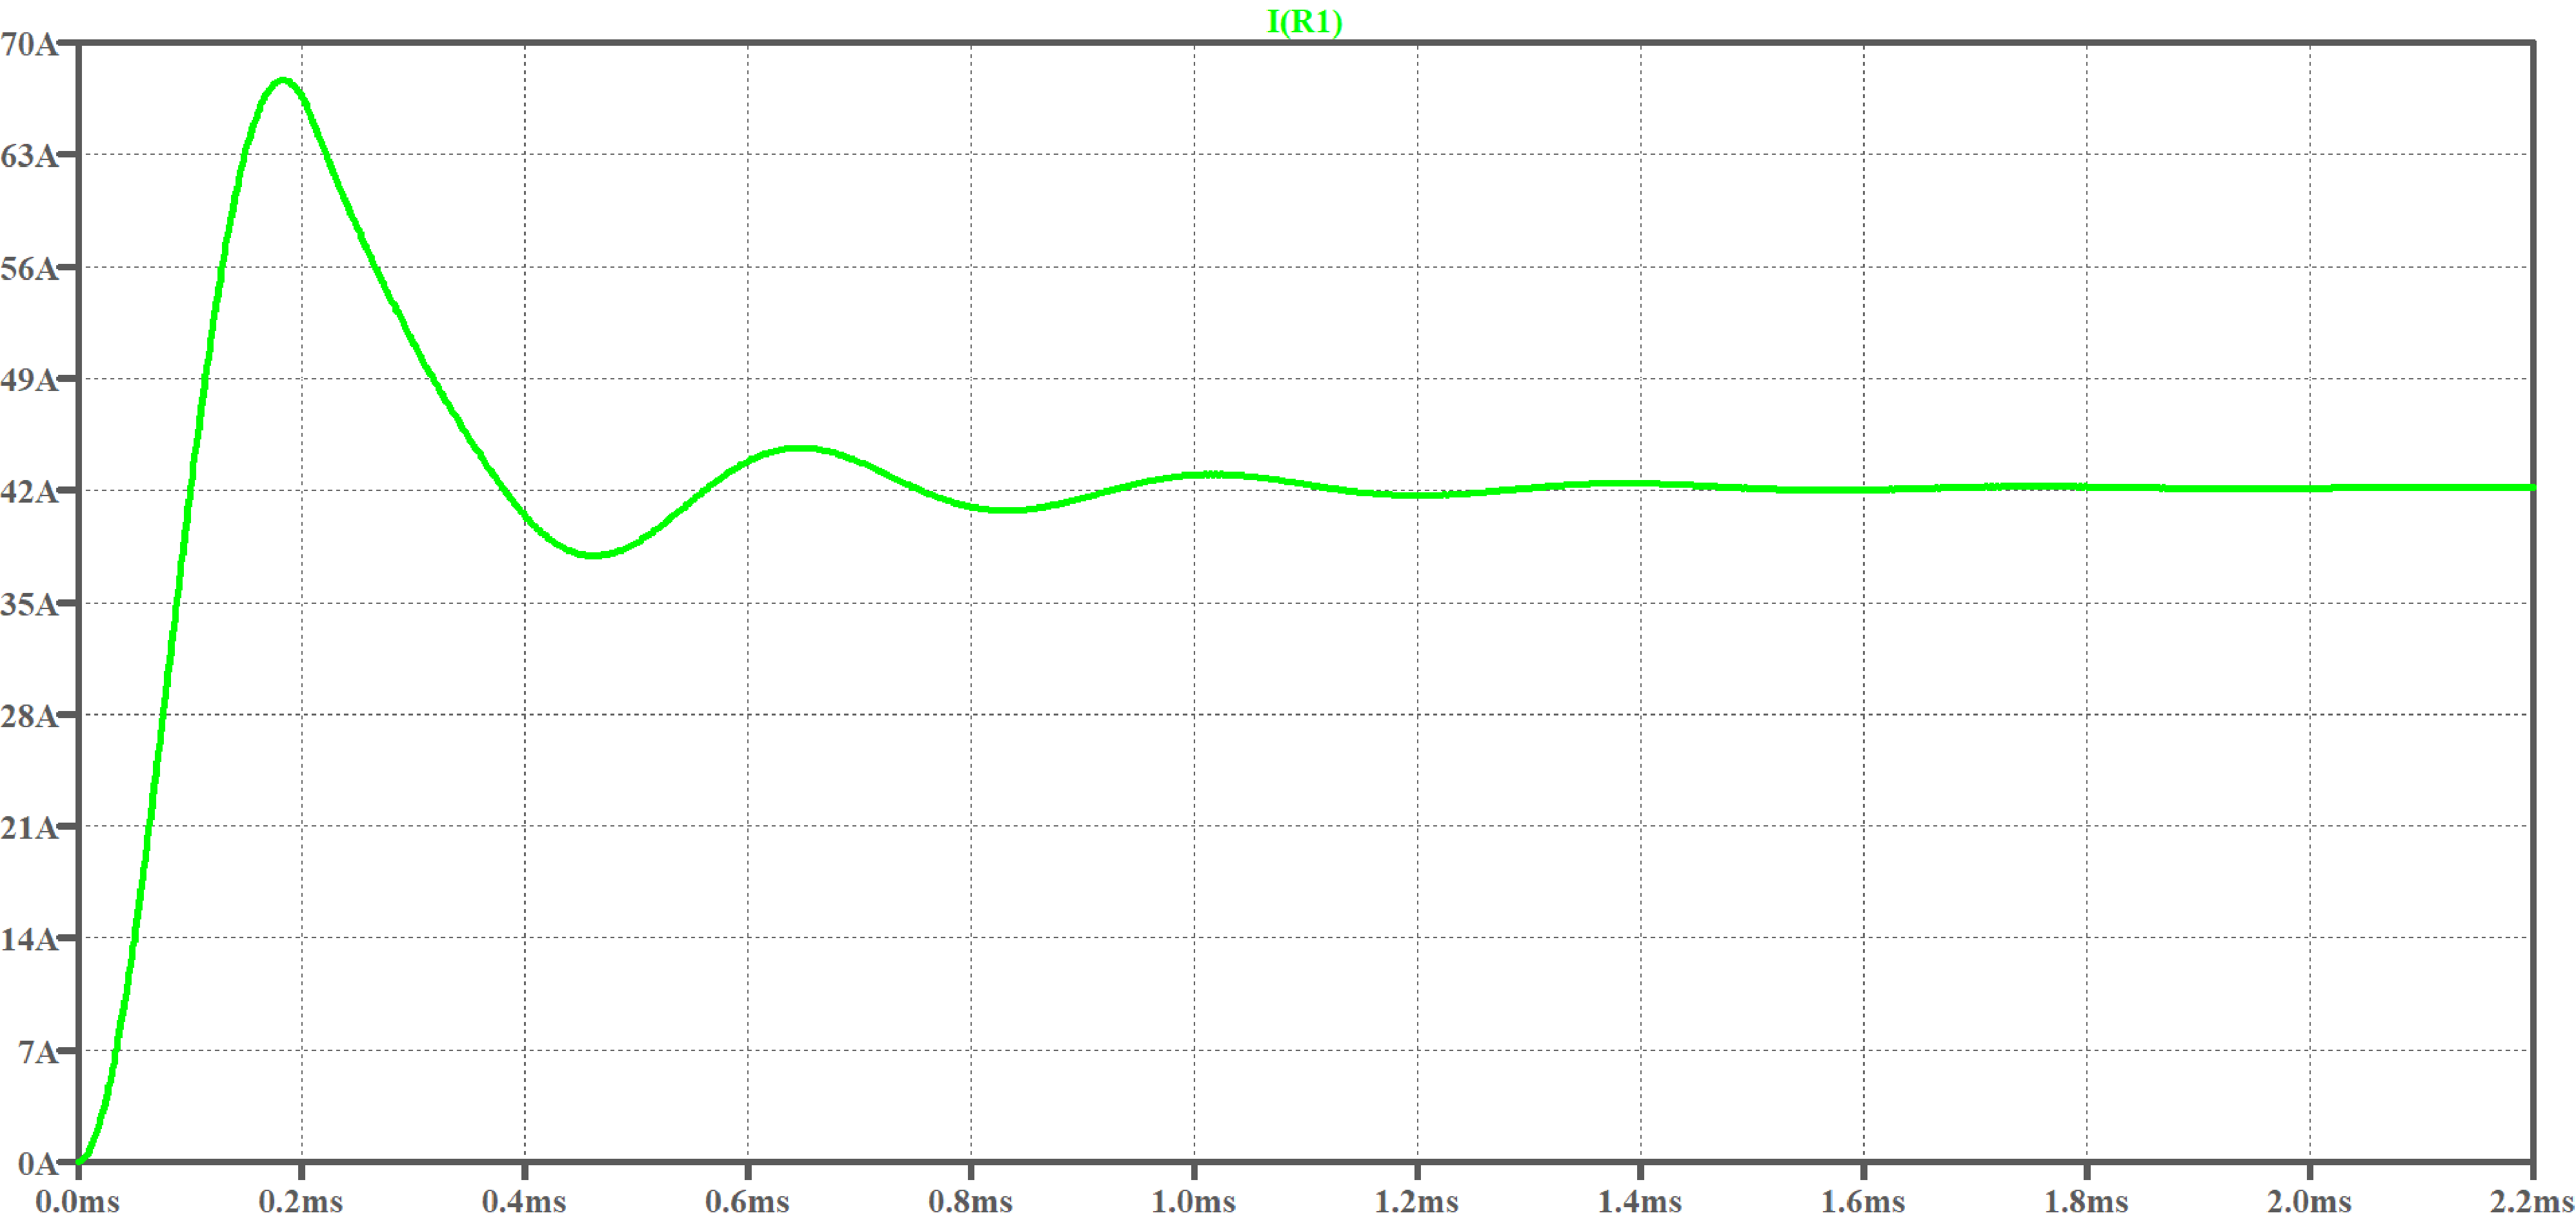
\includegraphics[width=0.8\linewidth]{Pictures/image/output_current.pdf}
    \caption{\textcolor{blue}{\textit{\footnotesize Output Current Waveform}}}
\end{figure}
\newpage
\begin{figure}[h!]
    \centering
    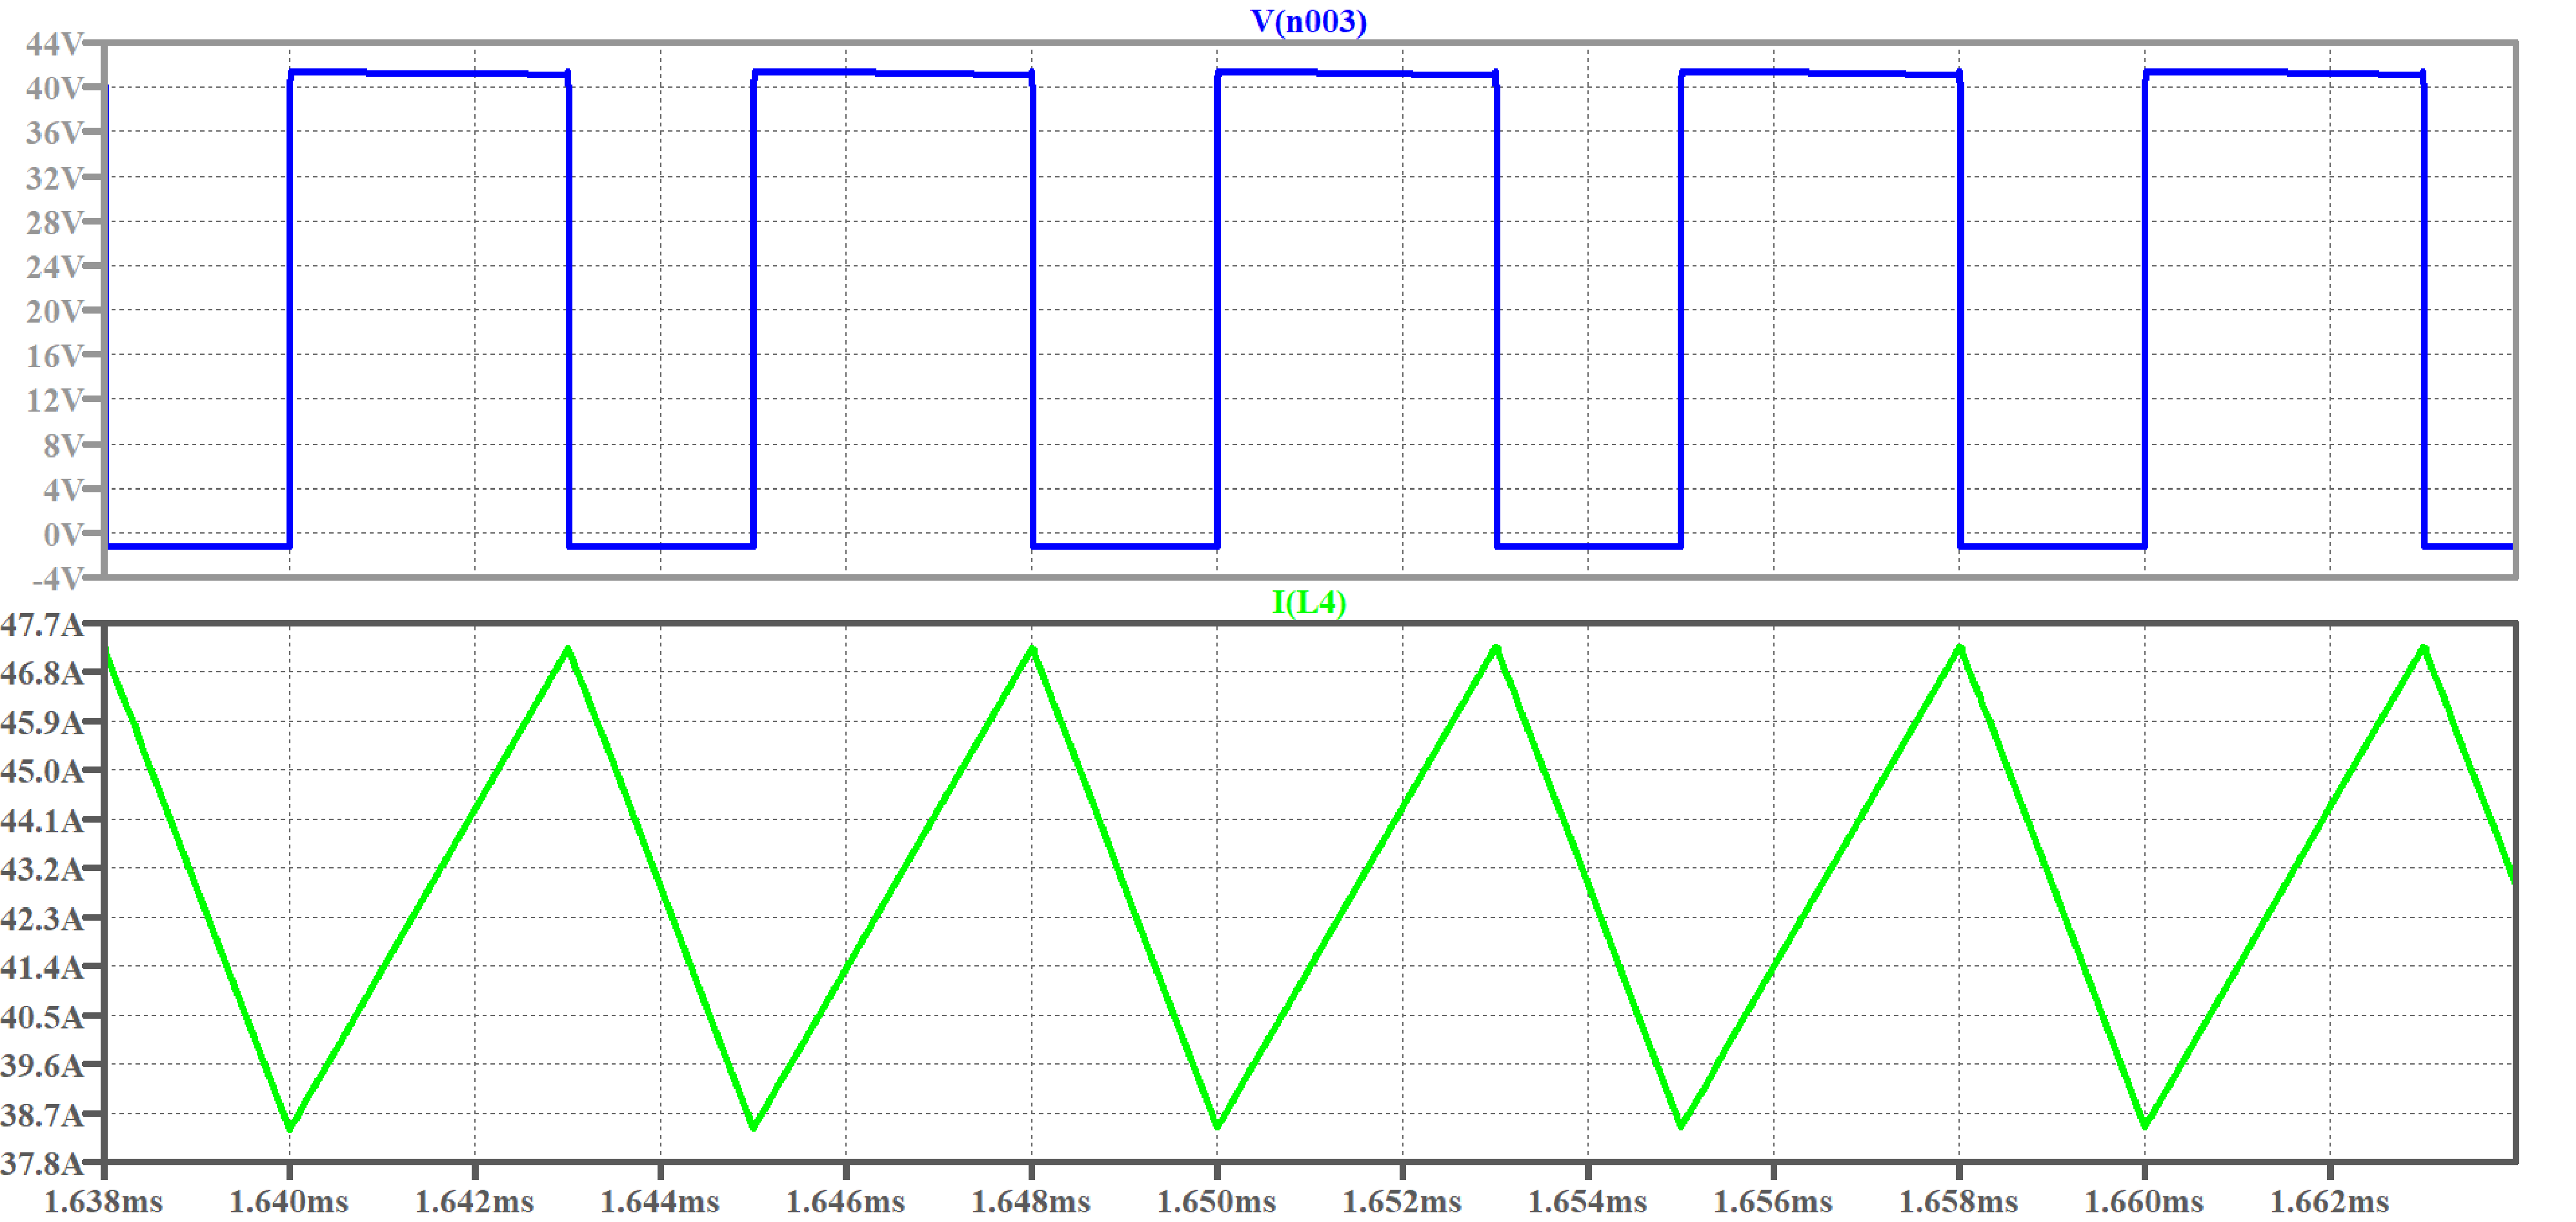
\includegraphics[width=0.8\linewidth]{Pictures/image/inductor_current.pdf}
    \caption{\textcolor{blue}{\textit{\footnotesize  Secondary Voltage and Inductor Current Waveform}}}
\end{figure}
\begin{figure}[h!]
    \centering
    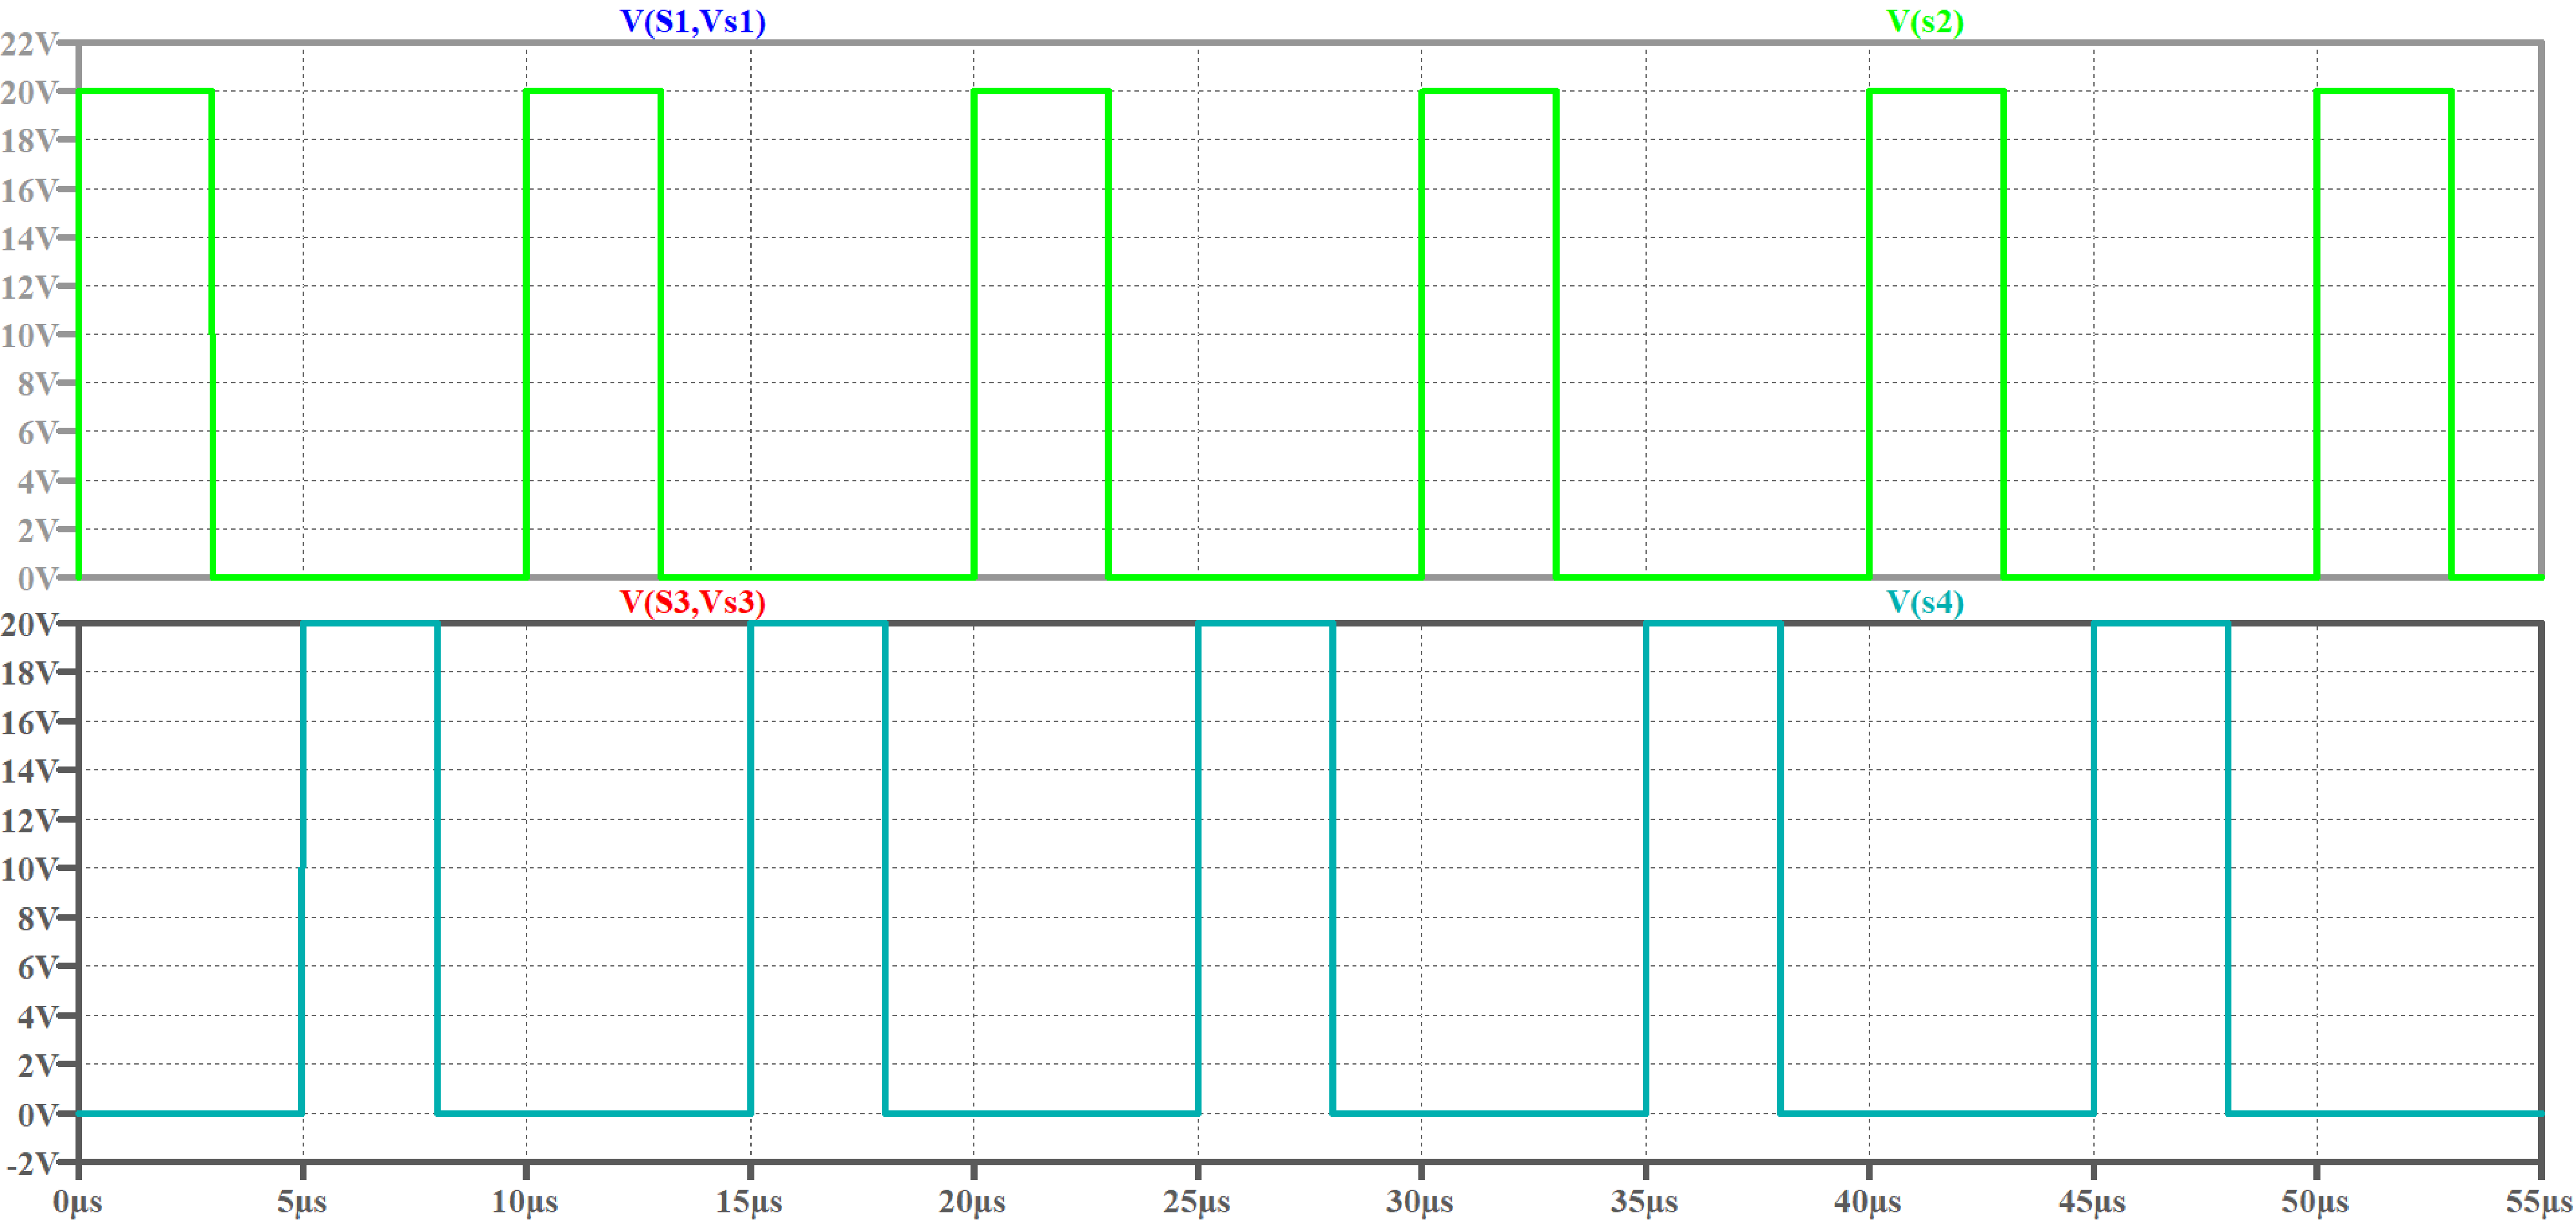
\includegraphics[width=0.8\linewidth]{Pictures/image/duty_s1_s2.pdf}
    \caption{\textcolor{blue}{\textit{\footnotesize Duty Cycle of S1 and S2}}}
\end{figure}


















% \begin{table}[h!]
% \centering
% \caption{Input Parameters for Transformer Design}
% \begin{tabular}{llll}
% \toprule
% \textbf{Parameter} & \textbf{Value} & \textbf{Parameter} & \textbf{Value} \\ \midrule
% $P_{\text{out}}$ & $\SI{500}{\watt}$ & $K_f$ & $4$ \\
% $V_{\text{in}}$ & $\SI{310}{\volt}$ & $B_m$ & $\SI{0.05}{\tesla}$ \\
% $U$ & $1.41$ & $F_{\text{sw}}$ & $\SI{100e3}{\hertz}$ \\
% $n$ & $0.9$ & $\alpha$ & $0.5$ \\
% $K_u$ & $0.4$ & $D$ & $0.3$ \\
% $I_{\text{out}}$ & $\SI{20.83}{\ampere}$ & & \\ \bottomrule
% \end{tabular}
% \end{table}
% \subsubsection*{Secondary Apparent Power (\(P_t\))}
% \begin{equation}
% P_t = \frac{P_{\text{out}}}{n} \cdot U = \frac{500}{0.9} \cdot 1.41 = \boxed{\SI{783.33}{\volt\ampere}}
% \end{equation}

% \subsubsection*{Electrical Condition (\(K_e\))}
% \begin{equation}
% K_e = 0.145 \cdot K_f^2 \cdot F_{\text{sw}}^2 \cdot B_m^2 \cdot 10^{-4} 
% = 0.145 \cdot 4^2 \cdot (100\text{e}3)^2 \cdot (0.05)^2 \cdot 10^{-4} 
% = \boxed{5800}
% \end{equation}

% \subsubsection*{Core Geometry (\(K_g\))}
% \begin{equation}
% K_g = \frac{P_t}{2 \cdot K_e \cdot \alpha} \cdot 1.35 
% = \frac{783.33}{2 \cdot 5800 \cdot 0.5} \cdot 1.35 
% = \boxed{\SI{0.182}{\centi\meter\tothe{5}}}
% \end{equation}

% \begin{figure}[h!]
%     \centering
%     
\includegraphics[width=1\linewidth]{Pictures/pics/PQ_CORE_500W.pdf}
%     \caption{\textcolor{blue}{\textit{\footnotesize PQ Core Parameter Table List}}}
% \end{figure} 
% \newpage
% \begin{figure}[h!]
%     \centering
%     
\includegraphics[width=1\linewidth]{Pictures/pics/PQ_CORE_STRUCTURE.pdf}
%     \caption{\textcolor{blue}{\textit{\footnotesize PQ32/30 Core}}}
% \end{figure} 


% \begin{table}[h!]
% \centering
% \caption{Core Parameters for Transformer Design}
% \begin{tabular}{llll}
% \toprule
% \textbf{Parameter} & \textbf{Value} & \textbf{Parameter} & \textbf{Value} \\ \midrule
% MPL & $\SI{7.46}{\centi\meter}$ & We & $\SI{55}{\gram}$ \\
% MLT & $\SI{6.7}{\centi\meter}$ & $A_c$ & $\SI{1.61}{\centi\meter\squared}$ \\
% $W_a$ & $\SI{1.496}{\centi\meter\squared}$ & $A_p$ & $\SI{2.409}{\centi\meter\tothe{4}}$ \\
% $K_{\text{gs}}$ & $\SI{0.2326}{\centi\meter\tothe{5}}$ & & \\ \bottomrule
% \end{tabular}
% \end{table}

% \subsubsection*{ Current Density (\(J\))}
% \begin{equation}
% J = \frac{P_t \cdot 10^4}{K_f \cdot K_u \cdot B_m \cdot F_{\text{sw}} \cdot A_p} 
% = \frac{783.33 \cdot 10^4}{4 \cdot 0.4 \cdot 0.05 \cdot 100\text{e}3 \cdot 2.409} 
% = \boxed{\SI{406.4}{\ampere\per\centi\meter\squared}}
% \end{equation}

% \subsubsection*{ Primary Turns (\(N_p\))}
% \begin{equation}
% N_p = \frac{V_{\text{in}} \cdot 10^4}{K_f \cdot B_m \cdot F_{\text{sw}} \cdot A_c} 
% = \frac{310 \cdot 10^4}{4 \cdot 0.05 \cdot 100\text{e}3 \cdot 1.61} 
% = \boxed{96\ \text{turns}}
% \end{equation}

% \subsubsection*{ Input Current (\(I_{\text{in}}\))}
% \begin{equation}
% I_{\text{in}} = \frac{P_{\text{out}}}{V_{\text{in}} \cdot n} 
% = \frac{500}{310 \cdot 0.9} 
% = \boxed{\SI{1.45}{\ampere}}
% \end{equation}

% \subsubsection*{ Primary Wire Area (\(A_{\text{pw}}\))}
% \begin{equation}
% A_{\text{pw}} = \frac{I_{\text{in}} \cdot \sqrt{D}}{J} 
% = \frac{1.45 \cdot \sqrt{0.3}}{406.4} 
% = \boxed{\SI{0.00196}{\centi\meter\squared}}
% \end{equation}

% \subsubsection*{ Secondary Voltage (\(V_s\))}
% \begin{equation}
% V_s = \frac{V_{\text{in}}}{7.15} = \frac{310}{7.15} = \boxed{\SI{43.36}{\volt}}
% \end{equation}

% \subsubsection*{9. Secondary Turns (\(N_s\))}
% \begin{equation}
% N_s = \frac{N_p \cdot V_s}{V_{\text{in}}} \cdot \left(1 + \frac{\alpha}{100}\right) 
% = \frac{96 \cdot 43.36}{310} \cdot 1.005 
% = \boxed{13.5\ \text{turns}}
% \end{equation}

% \subsubsection*{ Secondary Wire Area (\(A_{\text{sw}}\))}
% \begin{equation}
% A_{\text{sw}} = \frac{I_{\text{out}} \cdot \sqrt{D}}{J} 
% = \frac{20.83 \cdot \sqrt{0.3}}{406.4} 
% = \boxed{\SI{0.028}{\centi\meter\squared}}
% \end{equation}

% \subsection{Output Inductor Design}
% \begin{table}[h!]
% \centering
% \caption{Input Parameters for Ferrite Core Selection}
% \begin{tabular}{ll}
% \toprule
% \textbf{Parameter} & \textbf{Value} \\ \midrule
% Inductance (\(L\)) & \(\SI{16e-6}{\henry}\) \\
% DC Current (\(I_o\)) & \(\SI{20.83}{\ampere}\) \\
% AC Ripple Current (\(\Delta I\)) & \(\SI{6.25}{\ampere}\) \\
% Output Power (\(P_o\)) & \(\SI{500}{\watt}\) \\
% Regulation (\(\alpha\)) & \(1\%\) \\
% Switching Frequency (\(F_s\)) & \(\SI{100e3}{\hertz}\) \\
% Flux Density (\(B_m\)) & \(\SI{0.25}{\tesla}\) \\
% Window Utilization (\(K_u\)) & \(0.4\) \\
% Temperature Rise (\(T_r\)) & \(\SI{25}{\celsius}\) \\ \bottomrule
% \end{tabular}
% \end{table}

% \subsubsection*{Peak Current}
% \begin{equation}
% \text{(\(I_{\text{pk}}\))} = I_o + \frac{\Delta I}{2} = 20.83 + \frac{6.25}{2} = \boxed{\SI{23.96}{\ampere}}
% \end{equation}

% \subsubsection*{Energy Handling}
% \begin{equation}
% \text{ (\(E\))} = \frac{1}{2} L I_{\text{pk}}^2 = \frac{1}{2} \cdot 16 \times 10^{-6} \cdot (23.96)^2 = \boxed{\SI{0.00459}{\joule}}
% \end{equation}

% \subsubsection*{Electrical Coefficient}
% \begin{equation}
% \text{ (\(K_e\))} = 0.145 \cdot P_o \cdot B_m^2 \cdot 10^{-4} 
% = 0.145 \cdot 500 \cdot (0.25)^2 \cdot 10^{-4}
% = \boxed{0.000453}
% \end{equation}

% \subsubsection*{Core Geometry}
% \begin{equation}
% K_g = \frac{E^2}{K_e \cdot \alpha} = \frac{(0.00459)^2}{0.000453 \cdot 1} = \boxed{\SI{0.0465}{\centi\meter\tothe{5}}}
% \end{equation}

% \begin{figure}[h!]
%     \centering
%     
\includegraphics[width=1\linewidth]{Pictures/pics/ETD_500W.pdf}
%     \caption{\textcolor{blue}{\textit{\footnotesize ETD Core Parameter Table List}}}
% \end{figure} 
% \begin{figure}[h!]
%     \centering
%     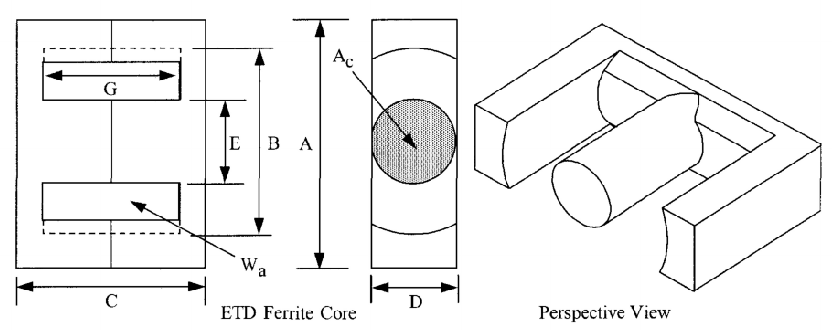
\includegraphics[width=1\linewidth]{Pictures/pics/ETD_CORE_STRUCTURE.pdf}
%     \caption{\textcolor{blue}{\textit{\footnotesize ETD-29 Core}}}
% \end{figure} 
% \subsubsection*{Current Density}
% \begin{equation}
%     J = \frac{2 \cdot E \cdot 10^4}{B_m \cdot A_p \cdot K_u} 
% = \frac{2 \cdot 0.008 \cdot 10^4}{0.25 \cdot 1.08 \cdot 0.4} = \boxed{\SI{1481.48}{\ampere\per\centi\meter\squared}}
% \end{equation}
% \subsubsection*{RMS Current}
% \begin{equation}
%     \text{2. RMS Current } I_{\text{rms}} = \sqrt{I_o^2 + (\Delta I)^2} \\
% = \sqrt{20.83^2 + 6.25^2} = \boxed{\si{21.75}\ \text{A}}
% \end{equation}
% \subsubsection*{Bare Wire Area}
% \begin{equation}
%  A_w = \frac{I_{\text{rms}}}{J} = \frac{21.75}{1481.48} = \boxed{\si{0.0147}\ \text{cm}^5}
% \end{equation}
% \subsubsection*{Selected Wire Area}
% \[
% A_{ws} = 0.02\ \text{cm}^2
% \]
% \subsubsection*{Effective Window Area}
% \begin{itemize}
%     \item $S_3 = 0.75$ Window Effective factor for Ferrite core
% \end{itemize}
% \begin{equation}
% W_{\text{aeff}} = W_a \cdot S_3 = 1.419 \cdot 0.75 = \boxed{\si{1.064}\ \text{cm}^2}
% \end{equation}
% \subsubsection*{Number of Turn}
% \begin{itemize}
%     \item $S_2 = 0.6$ Fill Factor 
% \end{itemize}
% \begin{equation}
% N = \frac{W_{a,eff} \cdot S_2}{A_{ws}} = \frac{1.064 \cdot 0.6}{0.02} = \boxed{\si{31.92}\ \text{turn}}   
% \end{equation}

% \subsubsection*{Required Air Gap}
% \begin{equation}
% L_g = \frac{0.4\pi N^2 A_c \cdot 10^{-8}}{L} - \frac{MPL}{\mu_0} =  \frac{0.4 \cdot \pi \cdot 31.92^2 \cdot 0.761 \cdot 10^{-8}}{16 \cdot 10^{-6}} = \boxed{\si{0.006}\ \text{cm}} 
% \end{equation}
% \subsection{Simulation On LTspice}
% \begin{figure}[h!]
%     \centering
%     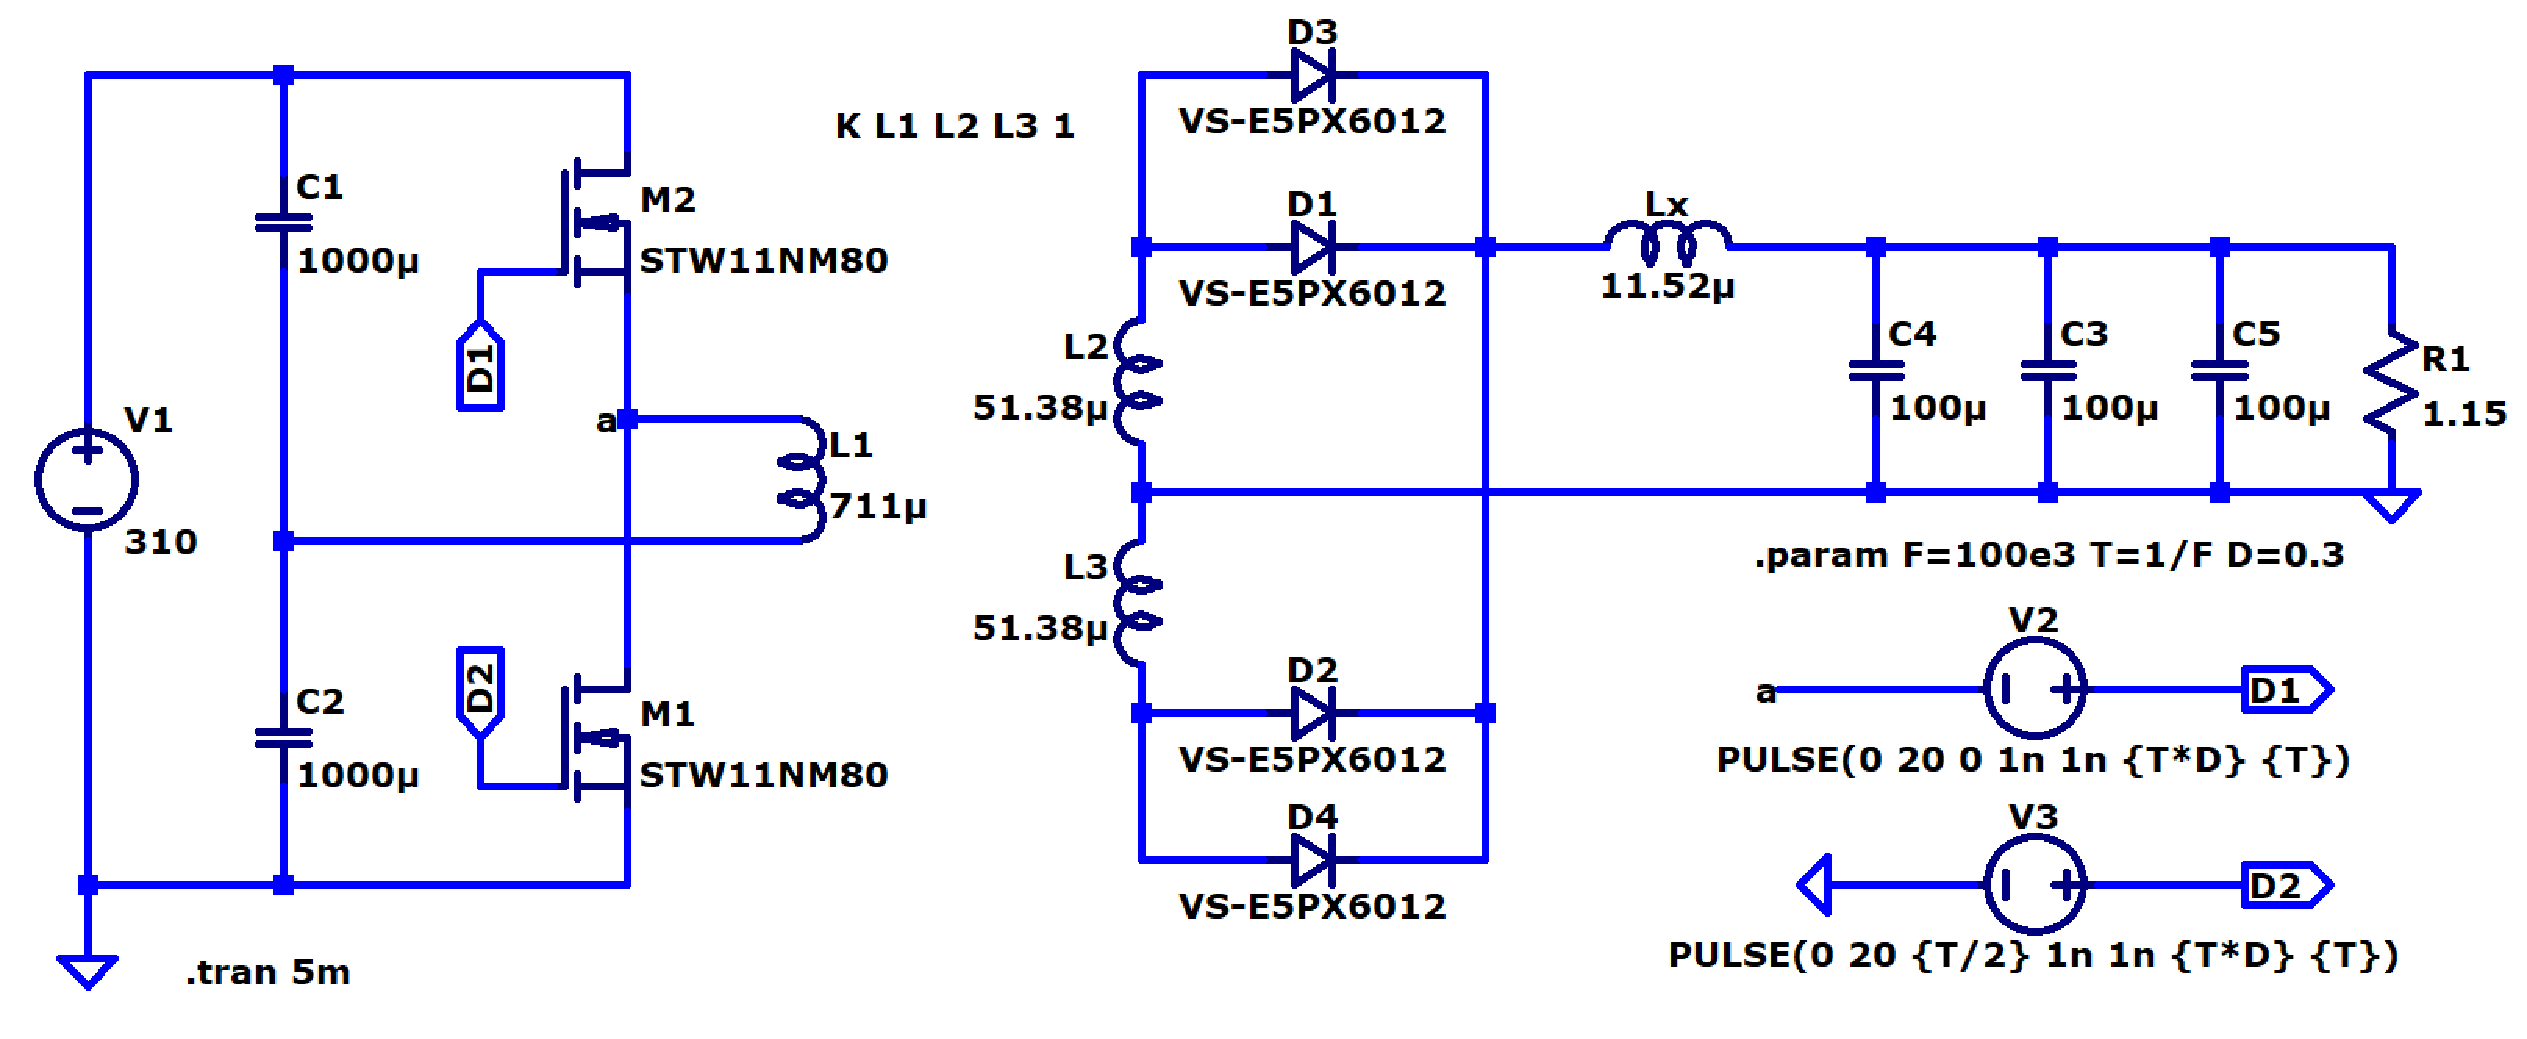
\includegraphics[width=1\linewidth]{Pictures/pics/lt_schem.pdf}
%     \caption{\textcolor{blue}{\textit{\footnotesize Push-Pull Converter Schematic on LTspice}}}
% \end{figure}
% \newpage
% \begin{figure}[h!]
%     \centering
%     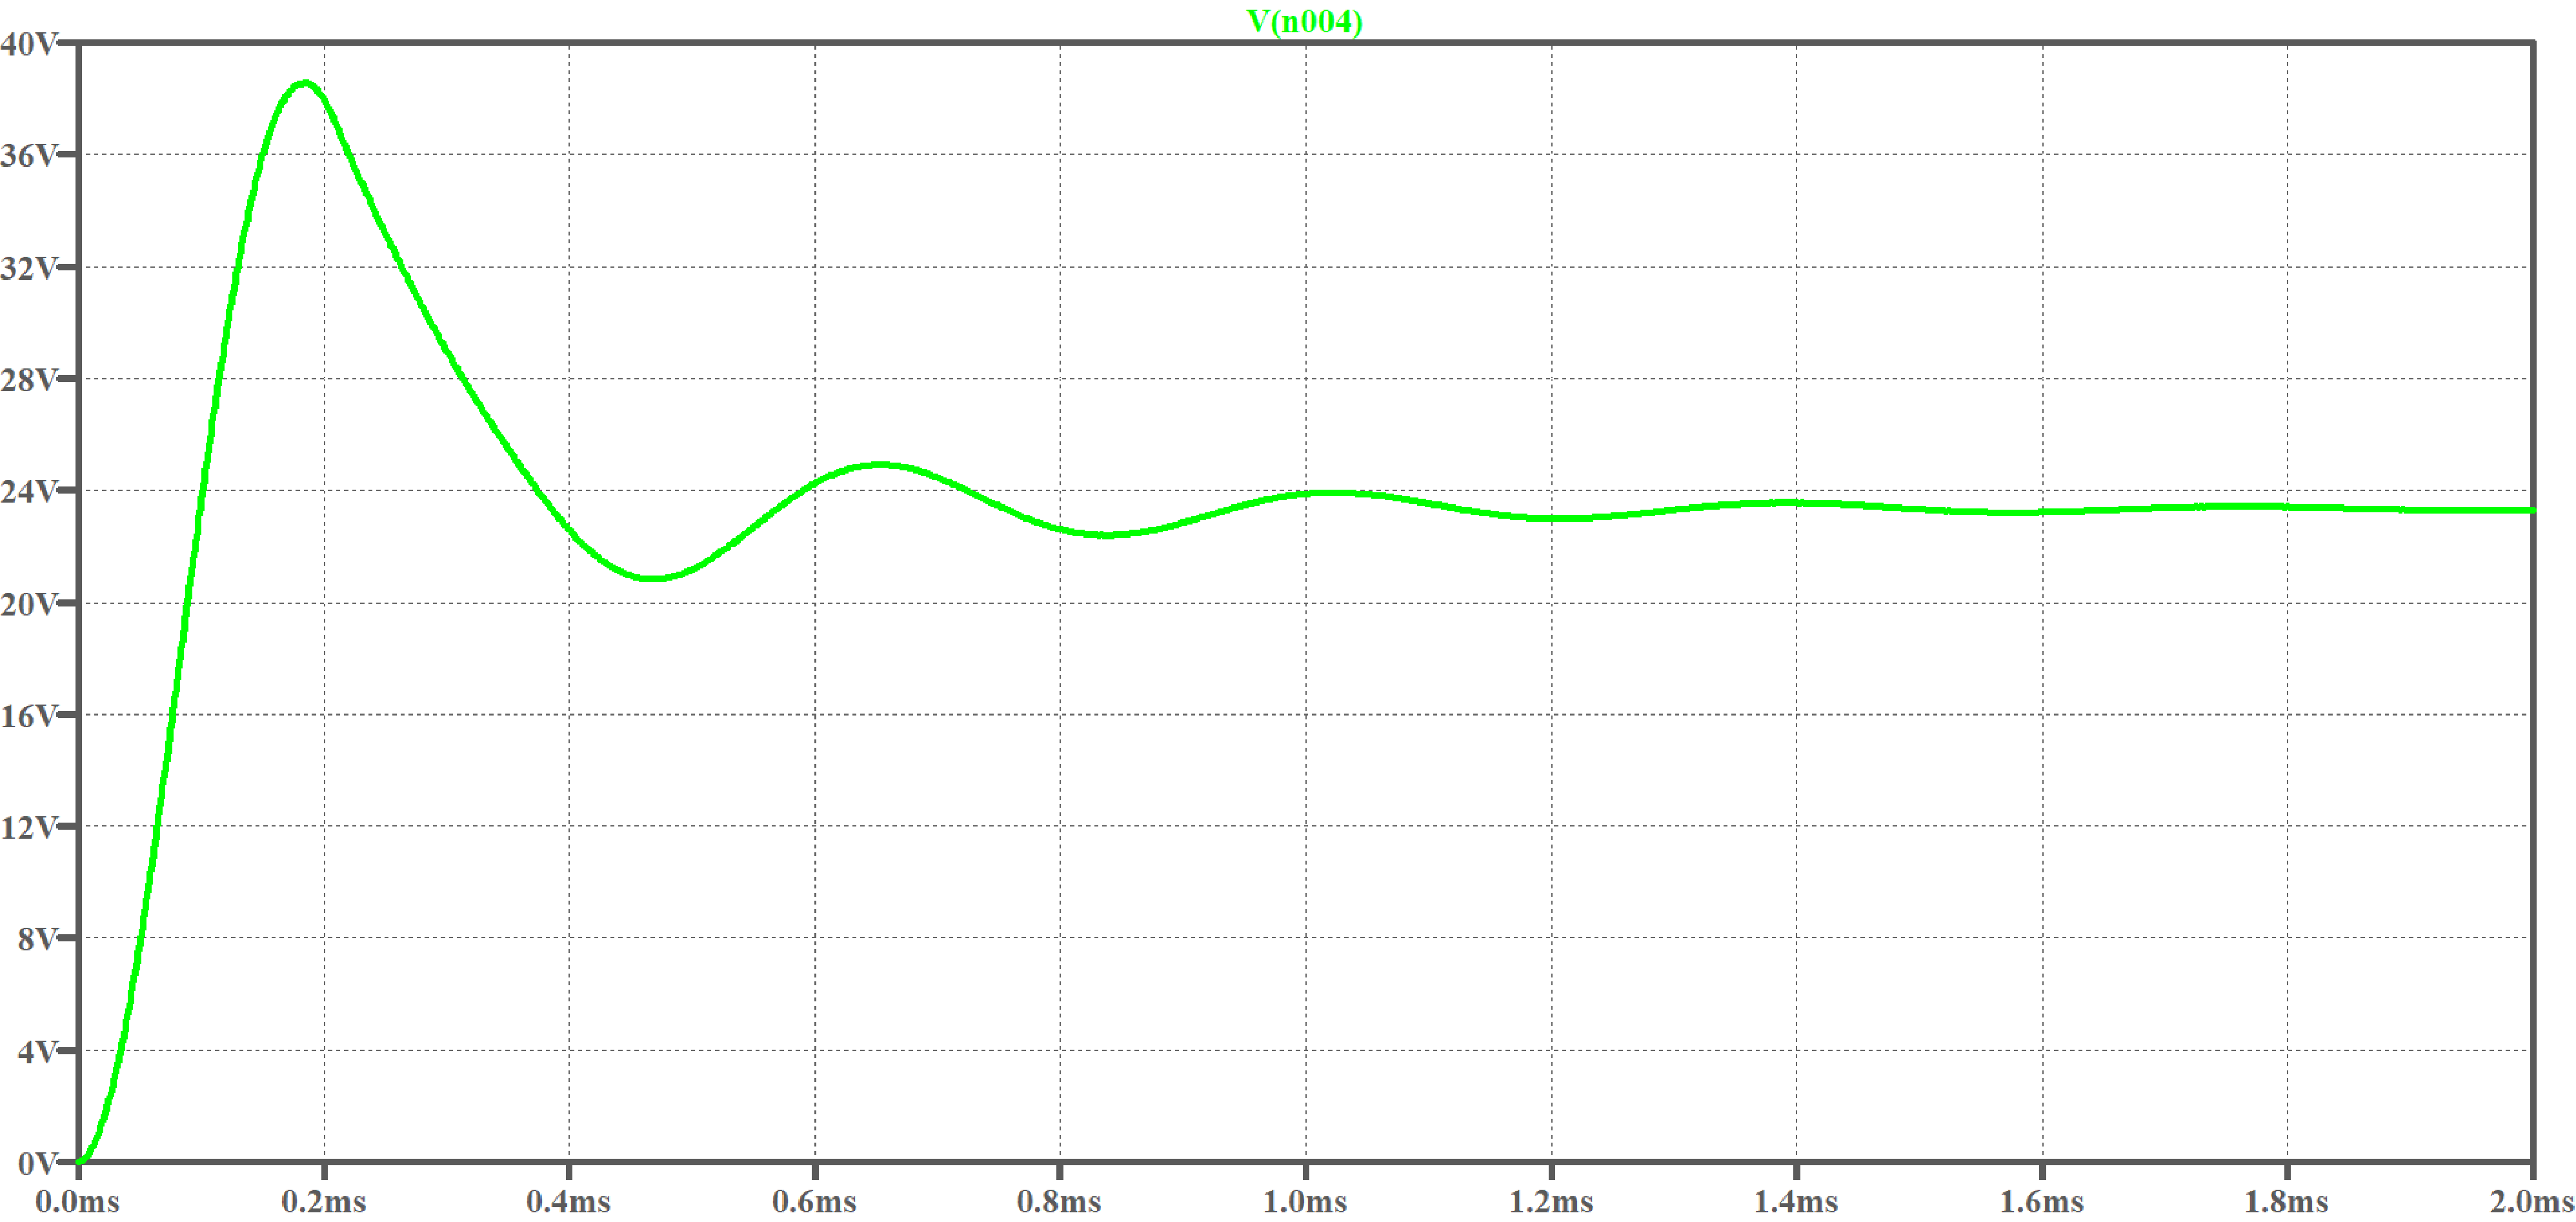
\includegraphics[width=0.8\linewidth]{Pictures/pics/lt_output_voltage.pdf}
%     \caption{\textcolor{blue}{\textit{\footnotesize Output Voltage Waveform}}}
% \end{figure}
% \begin{figure}[h!]
%     \centering
%     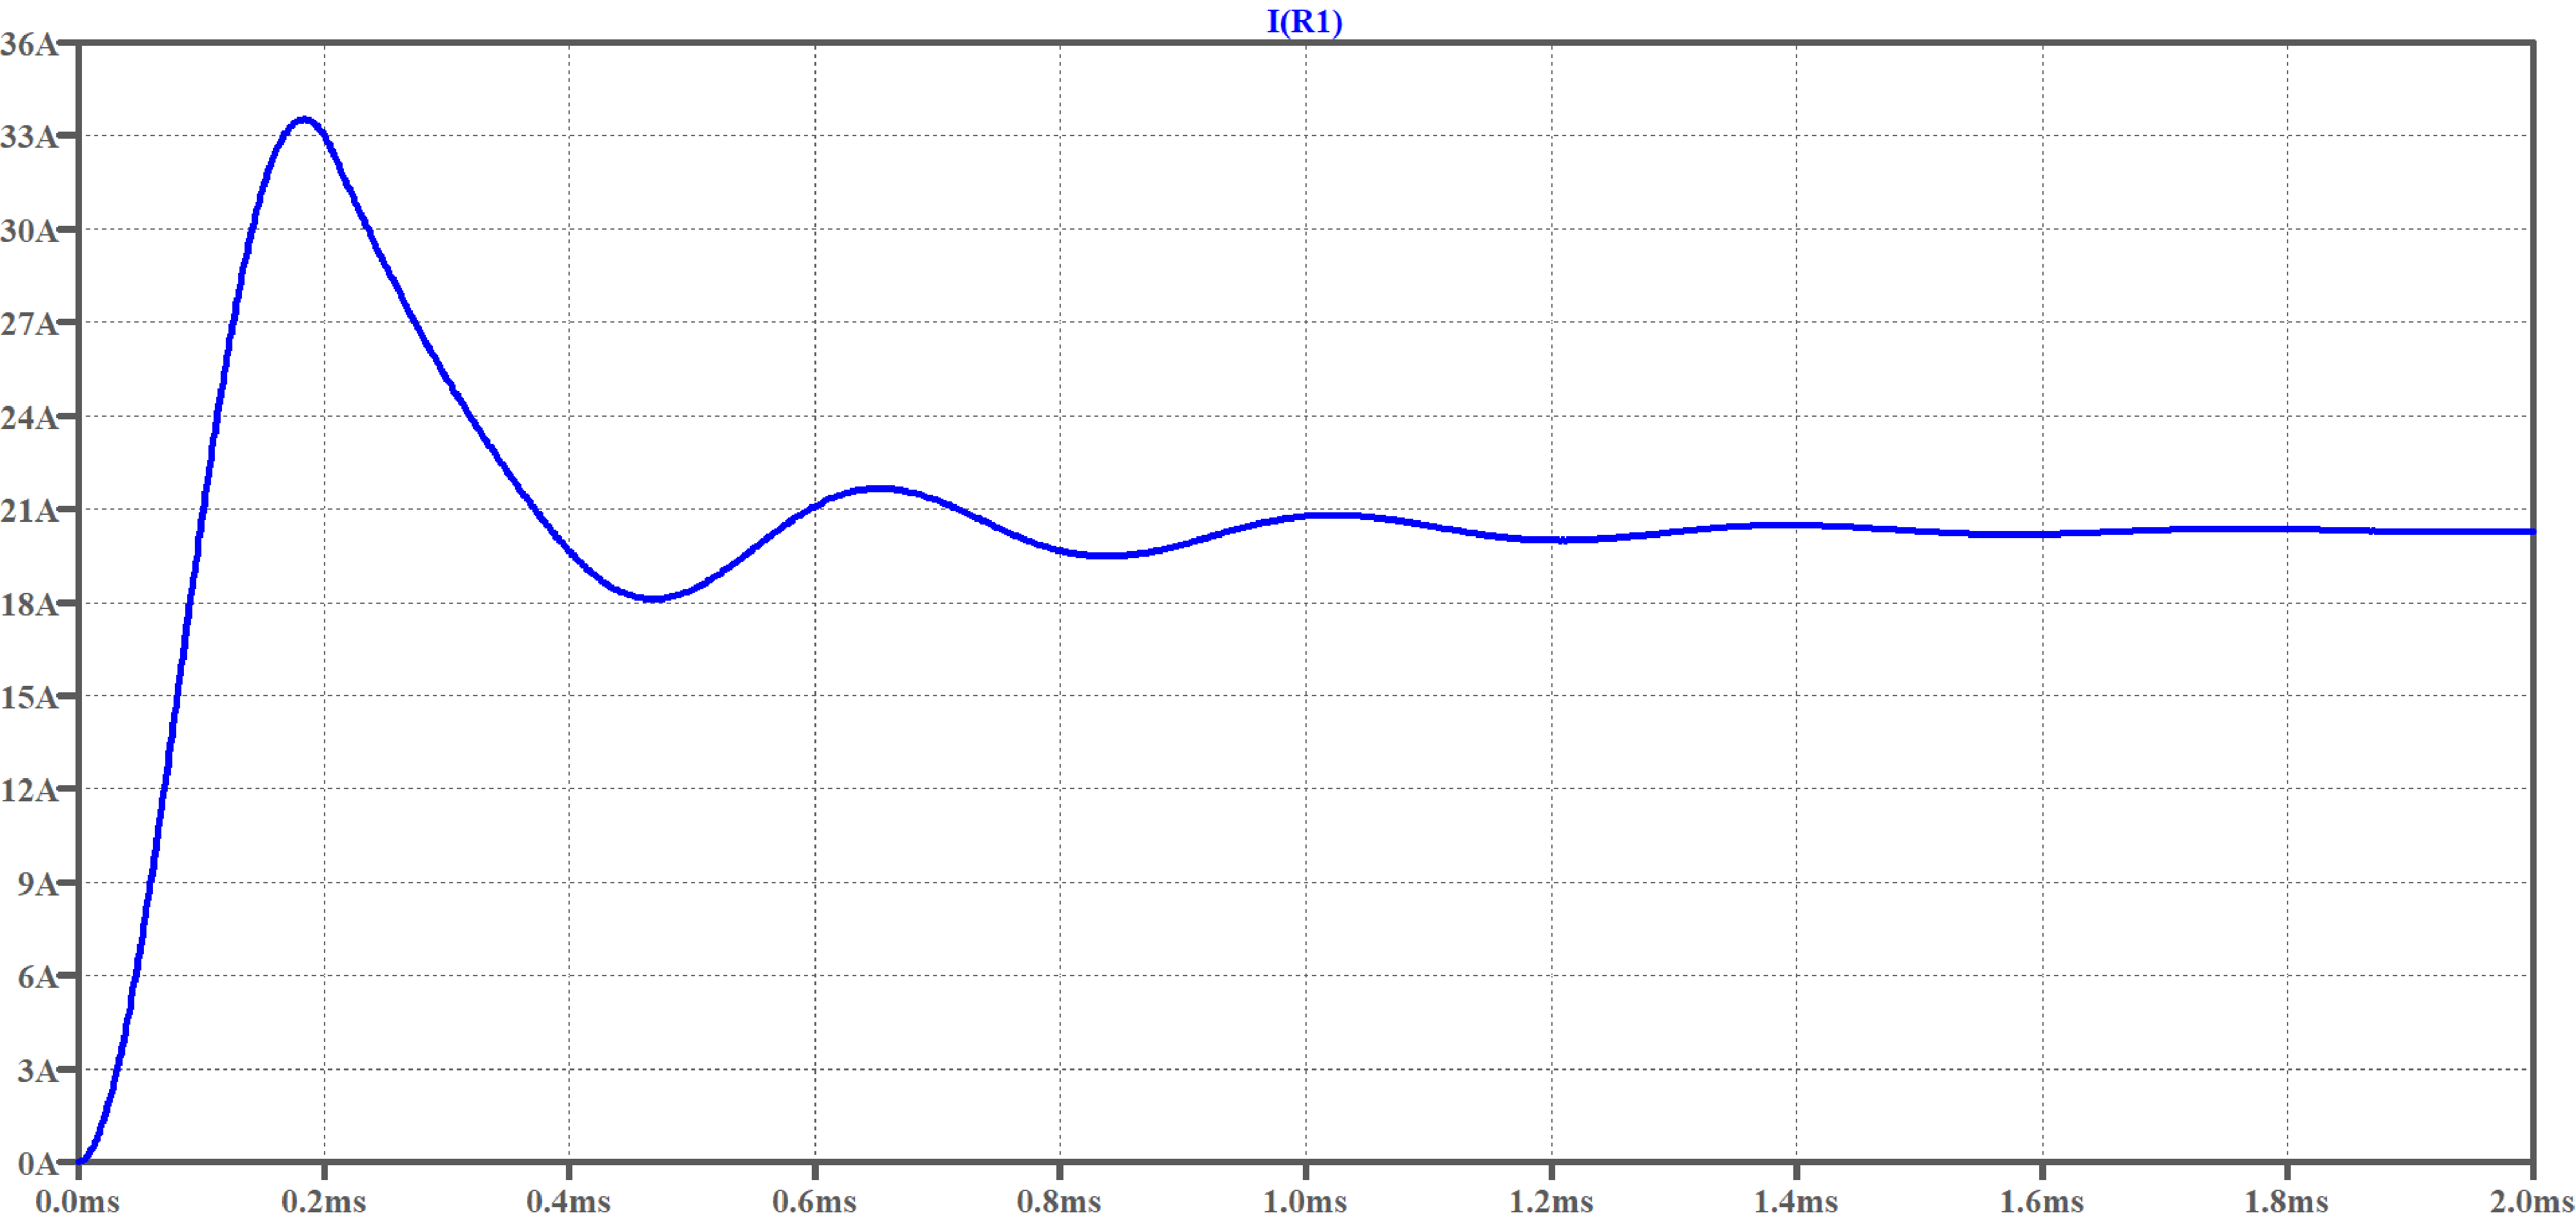
\includegraphics[width=0.8\linewidth]{Pictures/pics/lt_output_current.pdf}
%     \caption{\textcolor{blue}{\textit{\footnotesize Output Current Waveform}}}
% \end{figure}
% \begin{figure}[h!]
%     \centering
%     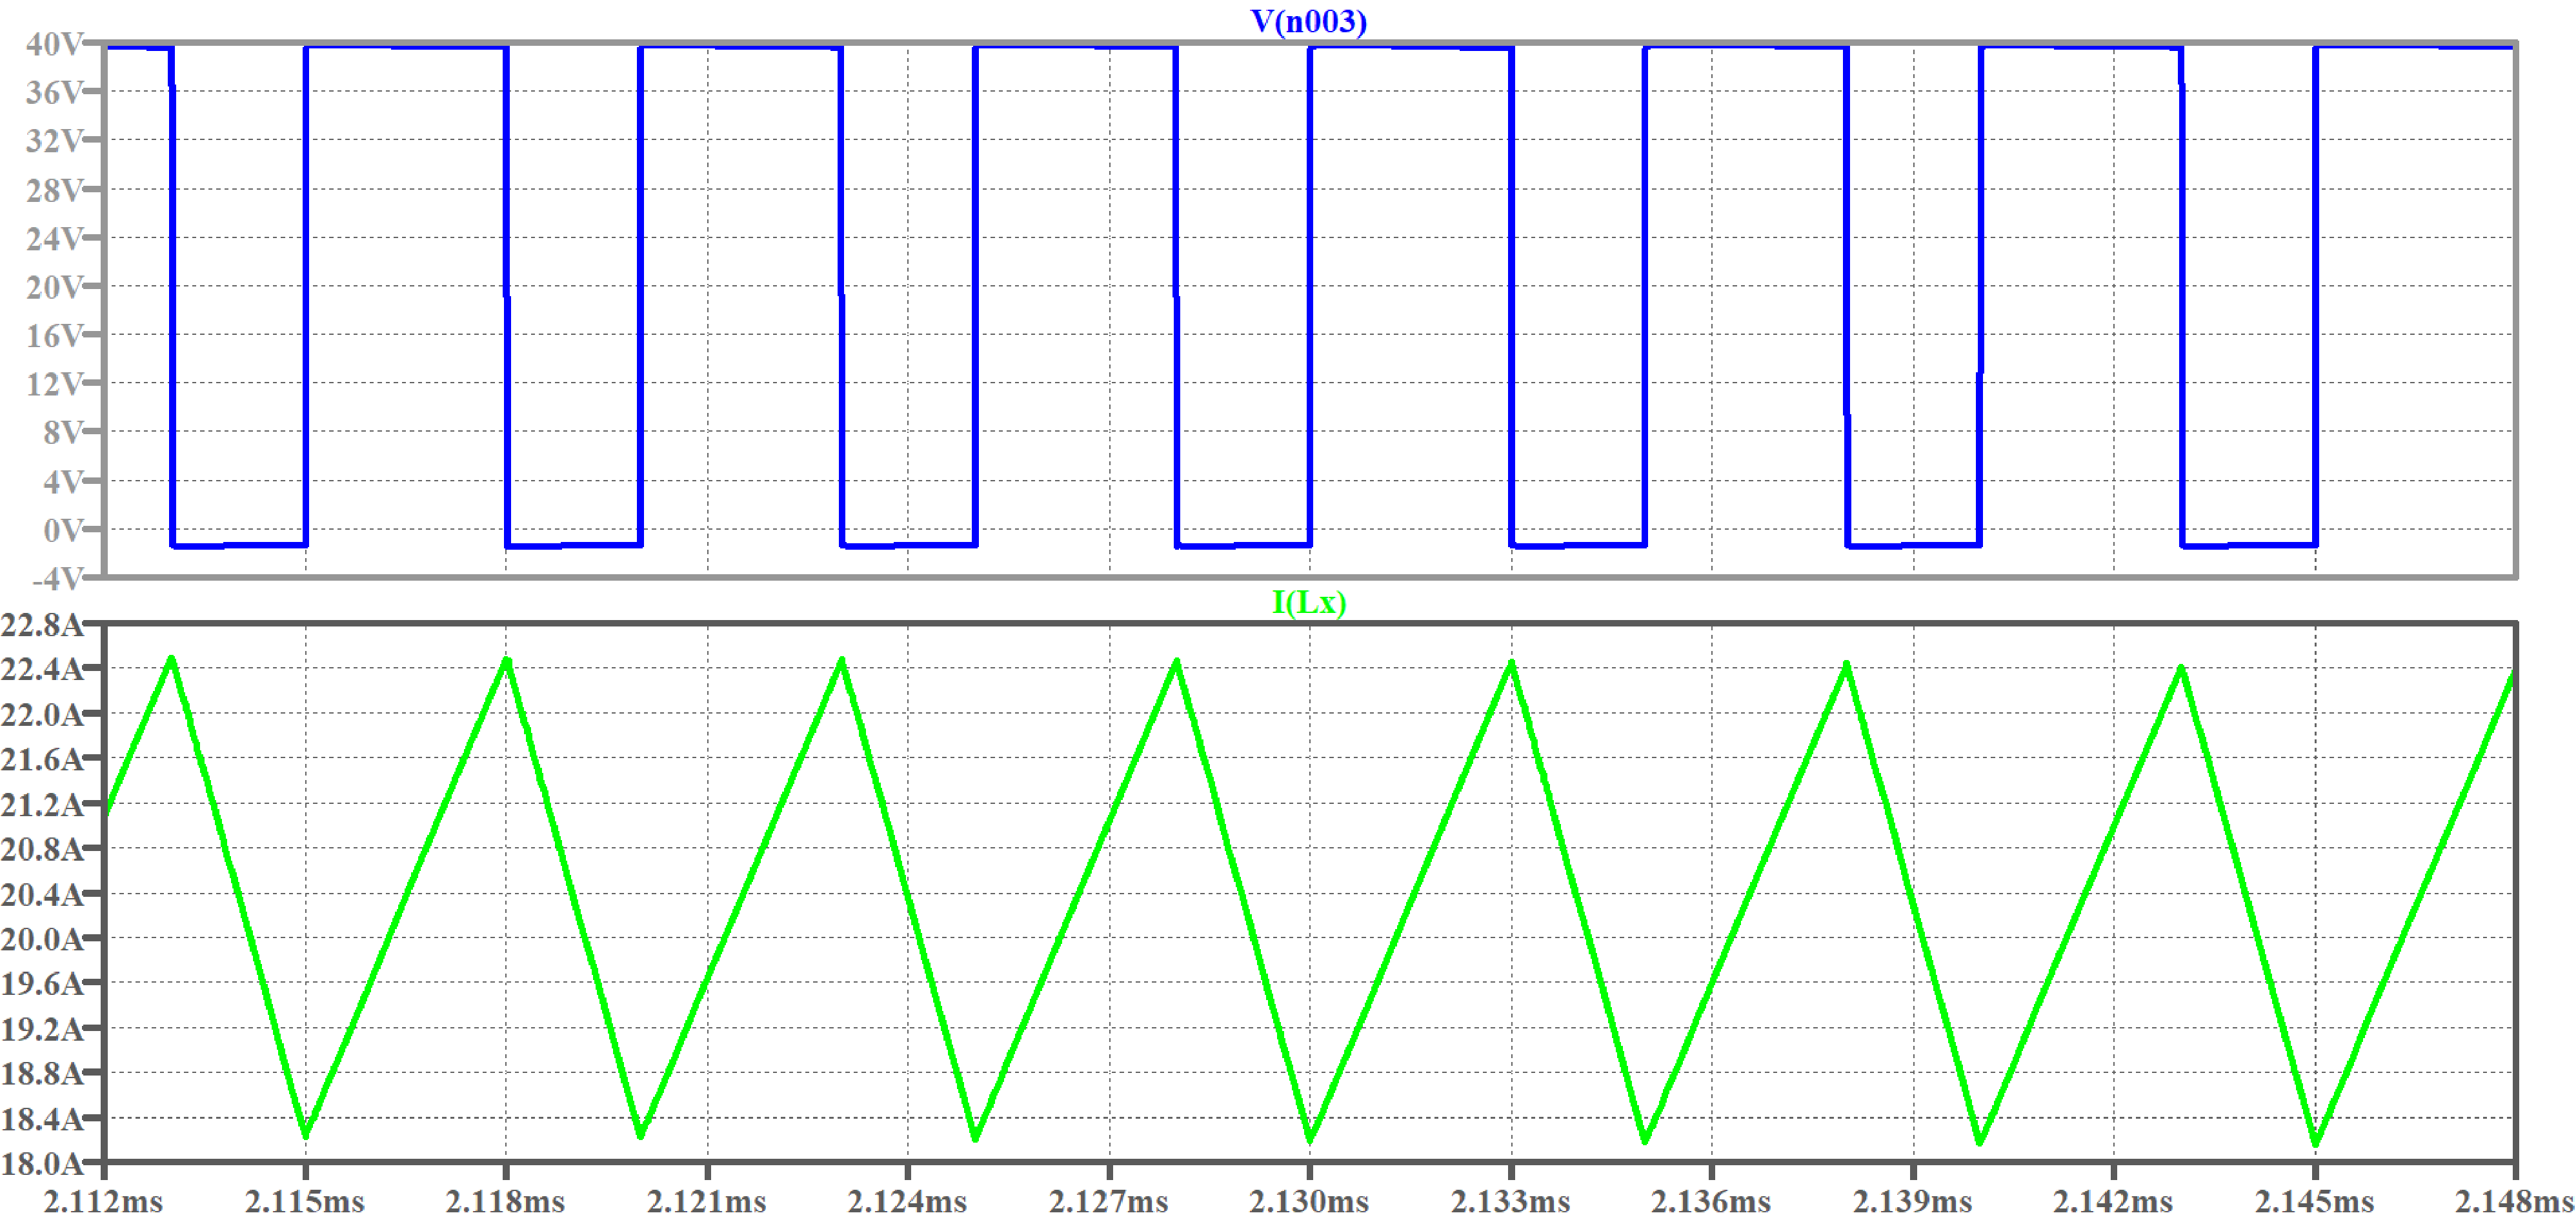
\includegraphics[width=0.8\linewidth]{Pictures/pics/lt_inductor_current.pdf}
%     \caption{\textcolor{blue}{\textit{\footnotesize  Secondary Voltage and Inductor Current Waveform}}}
% \end{figure}
% \newpage
% \begin{figure}[h!]
%     \centering
%     
\includegraphics[width=0.8\linewidth]{Pictures/pics/lt_duty_cycle.pdf}
%     \caption{\textcolor{blue}{\textit{\footnotesize Duty Cycle of S1 and S2}}}
% \end{figure}
